% !TeX encoding = UTF-8
% !TeX program = pdflatex
% !TeX spellcheck = it_IT

\documentclass[Lau,binding=0.6cm]{sapthesis}

\usepackage{verbatim}  % Needed for the "comment" environment to make LaTeX comments
\usepackage{vector}  % Allows "\bvec{}" and "\buvec{}" for "blackboard" style bold vectors in maths
\usepackage{bytefield}
\usepackage{amsmath}
\usepackage{amssymb}
\usepackage{float}
\usepackage{graphicx}
\usepackage{subfig}
\usepackage{caption}


\usepackage[maxbibnames=99]{biblatex}
\addbibresource{Bibliografia.bib}

\usepackage{microtype}
\usepackage[italian]{babel}
\usepackage[utf8]{inputenx}
\usepackage{csquotes}


\usepackage{hyperref}
\hypersetup{pdftitle={Sapthesis class example},pdfauthor={Francesco Biccari}}

% Remove in a normal thesis
\usepackage{lipsum}
\usepackage{curve2e}
\definecolor{gray}{gray}{0.4}
\newcommand{\bs}{\textbackslash}

% Commands for the titlepage
\title{Protocollo di localizzazione per reti di sensori sottomarini}
\author{Andrea Monterubbiano}
\IDnumber{1378872}
\course{Informatica}
\courseorganizer{Facoltà di Ingegneria dell'Informazione, Informatica e Statistica}
\AcademicYear{2017/2018}
\copyyear{2017}
\advisor{Prof. Chiara Petrioli}

\authoremail{andrea.monterubbiano@gmail.com}

\examdate{25 Ottobre 2017}
\examiner{Prof. Nome Cognome}
\examiner{Prof. Nome Cognome}
\examiner{Dr. Nome Cognome}
\versiondate{\today}



\begin{document}

\frontmatter

\maketitle

\dedication{Dedicato a\\ Donald Knuth}

\begin{abstract}

\end{abstract}

\begin{acknowledgments}
Ho deciso di scrivere i ringraziamenti in italiano
per dimostrare la mia gratitudine verso i membri
del GuIT, il Gruppo Utilizzatori Italiani di \TeX, e, in particolare,
verso il prof. Enrico Gregorio.
\end{acknowledgments}

\tableofcontents

\mainmatter

% Do not use the starred version of the chapter command!
\chapter{Introduzione}

\section{Reti Sottomarine}
Introduciamo il concetto di UWSNs, ovvero Underwater Wireless  Sensor Networks, con il quale intendiamo definire una rete di sensori e veicoli, di diversa natura ed in numero variabile, disposti in una limitata area sottomarina e capaci, in maniera collaborativa, di realizzare una missione che imponga la necessità di comunicare fra i diversi componenti della rete.\\
I diversi nodi della rete, la cui natura puo' variare da sensori fissati al fondale marino a veri e propri veicoli sottomarini autonomi (Autonomous Underwater Vehicle, AUV), debbono spesso possedere la capacità di adattarsi in maniera autonoma alle caratteristiche cangianti dell'ambiente in cui vengono utilizzati, scambiando fra loro ed elaborando informazioni riguardo posizionamento, movimento dei nodi mobili e configurazione propria di ciascuno di essi, al fine di coordinare efficacentemente il proprio lavoro e, se necessario, comunicare dati utili alle postazioni sulla terraferma.

\subsection{Applicazioni delle UWSNs}
Le reti sottomarine trovano applicazione in vari contesti, dalla raccolta di dati scientifici al monitoraggio e sorveglianza di una data area sottomarina, fino all'utilizzo nell'ambito dell'archeologia subacquea \cite{underwater}.\newline
Riportiamo un breve elenco delle situazioni d'utilizzo comuni per questo tipo di tecnologia:\newline
\begin{itemize}
\item Monitoraggio Ambientale:  \newline
Raccolta di dati riguardanti le caratteristiche fisiche, chimiche e biologiche di un area marina, al fine di valutarne il livello d'inquinamento e l'effetto dell'attività umana sull'ecosistema marino\newline
\item Esplorazione del fondale marino: \newline
Esplorazione subacquea con finalità di ricerca di riserve di combustibili fossili e posizionamento cavi sottomarini per telecomunicazioni\newline
\item Prevenzione di disastri:\newline
Monitoraggio di aree ad alto rischio sismico/vulcanico, in modo da poter studiare più efficacemente questi fenomeni naturali e poter disporre di un meccanismo d'allarme per le zone costiere in caso di tsunami\newline
\item Assitenza alla navigazione: \newline
Identificazione degli elementi di pericolo alla navigazione (scogli, fondali bassi, relitti affondati)\newline
\item Sorveglianza:\newline
Reti di nodi fissi e AUVs possono effettuare il monitoraggio di un'area assegnata provvedendo a compiti di sorveglianza, riconoscimento di oggetti all'interno dell'area, individuazione di obbiettivi sensibili e rilevamento di intrusi all'interno dell'area
\end{itemize}
Rispetto alle tecnologie preesistenti in questi campi d'azione (sistemi radar/sonar), queste reti di sensori sottomarini possono ricorrere ad un più ampio spettro qualitativo di dati (provenienti da sensori acustici, di radiazioni, di campi magnetici, sensori meccanici), raggiungendo un piu' alto grado di accuratezza nella rilevazione e classificazione di oggetti all'interno dell'area di sorveglianza.\newline

\subsection{Caratteristiche peculiari delle UWNSs e principali difficoltà progettuali}
Gli approcci tradizionali per la progettazione di sistemi che realizzano le funzioni sopra elencate sono accumunati da un approccio architetturale basato sul dispiegamento di sensori fissi, la raccolta di dati per un certo lasso di tempo, il recupero dei sensori e la successiva analisi dei dati accumulati.\newline
Le UWNSs ovviano ad alcuni limiti di questa tipologia di sistemi, nello specifico: \newline
\begin{itemize}
\item Introducono la possibilità di effettuare monitoraggio ed analisi dei dati in real-time, tramite la comunicazione dei dati a terra (caratteristica innovativa nei sistemi di monitoraggio di zone sismiche, ad esempio)\newline
\item L'interazione costante o cadenzata del personale scientifico con la rete di sensori ne permette la verifica per quanto riguarda il corretto funzionamento della strumentazione. \newline In questo modo si possono effettuare riconfigurazioni dei sistemi on-the-fly ed individuare eventuali malfunzionamenti dei sensori non appena questi si verificano (non dovendo più attendere il recupero dei sensori stessi)\newline
\item Viene meno la necessità di capacità di storage locali importanti per i sensori, avendo questi la possibilità di trasmettere i dati accumulati e quindi cancellarli per far posto ad altri rilevamenti
\end{itemize}
Le comunicazioni in questo tipo di reti avvengono solitamente tramite canale acustico. La scelta di questo tipo di trasmissione è praticamente obbligata dai limiti presenti nelle trasmissioni di tipo ottico ed elettromagnetico. Le prime soffrono di problemi legati a fenomeni di diffusione ottica.  Invece le onde elettromagnetiche, nel mezzo sottomarino, presentano un forte effetto di attenuazione, proporzionale alla distanza di trasmissione. La propagazione di onde elettromagnetiche in acqua per lunghe distanze potrebbe avvenire perciò solamente a frequenze molto basse (30-300 Hz), il che richiederebbe antenne ingombranti e un elevato dispendio energetico.

La trasmissione tramite onde acustiche si presenta quindi come l'unica soluzione tecnicamente avallabile nelle reti di comunicazione sottomarine. La peculiarità del mezzo, altresì, impone comunque particolare attenzione nella progettazione di protocolli di rete affidabili, a causa di alcune importanti limitazioni:
\begin{itemize}

\item La banda di trasmissione disponibile fortemente limitata

\item Fenomeni di trasmissione multi-path

\item Tasso di errore nella trasmissione elevato e frequente presenza di zone d'ombra

\item Disponibilità energetica limitata

\item Ritardo di propagazione altamente variabile e di cinque ordini di grandezza più elevato rispetto alle comunicazioni radio terrestri
\end{itemize}

Non ultimo va ricordato che il canale di comunicazione acustico è ovviamente da intendersi come canale ad accesso condiviso e, come anche le comunicazioni wireless elettromagnetiche, necessita di protocolli che gestiscano l'accesso concorrente al mezzo da parte di più nodi. Soluzioni che riprendono l'uso di pacchetti di tipo RTS e CTS, similarmente a quanto specificato dallo standard IEEE 802.11, non sono facilmente implementabili in ambiente underwater sia a causa dell'elevato delay che introdurrebbero (data la bassa capacità di una rete acoustica sottomarina) sia perchè sono molto piu' frequenti, rispetto alle normali reti wireless, fenomeni di "shadowing" temporaneo dei nodi della rete. Le ricerche recenti propendono invece per l'utilizzo di meccanismi di tipo TDMA e Slotted Aloha che, al costo di una bassa efficienza nell'utilizzo del canale e di una maggiore complessità d'implementazione, garantiscono l'accesso condiviso al canale senza la necessità di invio di pacchetti di controllo.



\subsection{Prospettiva sul ruolo dei dispositivi mobili nelle UWSNs}
I veicoli sottomarini stanno rivoluzionando l'approccio allo studio ed al monitoraggio dell'ambiente marino. \newline Sebbene questi veicoli necessitino di essere sganciati in acqua solitamente da una nave, una volta disposti nell'ambiente marino possono lavorare in maniera autonoma, non avendo necessita' di essere costantemente controllati dall'uomo durante le loro operazioni. \newline Questo ha permesso nel recente passato la realizzazione di missioni volte all'acquisizione di dati scientifici in zone altrimenti inaccessibili alla navigazione ( come ad esempio il deployment di AUVs sotto la lastra di ghiaccio artica \cite{wadhams}), migliorando inoltre la risoluzione spaziale e temporale rispetto a misurazioni effettuate in maniera indiretta.\newline
In questo paragrafo ci concentreremo sulla descrizione degli AUVs.
Come anticipato nel paragrafo percendente, gli AUVs sono veicoli sottomarini che non necessitano di equipaggio umano. Posseggono un proprio sistema di propulsione, vengono solitamente sganciati da una nave e possono operare indipendentemente da questa, per un periodo che va dalle ore all'ordine dei giorni. Molti degli AUVs sviluppati hanno la forma di siluro, sebbene ne esistano anche di forme diverse (adatti a particolari tipi di fondali e movimento).\newline
Il vantaggio principale degli AUVs rispetto ai gliders e' la possibilita' di navigare seguendo una traiettoria lineare, rendendoli adatti a missioni che richiedono il mantenimento di un'altezza costante.
Difatti, l'utilizzo piu' rilevante di questi veicoli  avviene in studi che riguardano la zona di interfacciamento del fondale marino con la colonna d'acqua soprastante o direttamente lo studio del fondale.  In questa zona dell'ambiente sottomarino si concentrano gli organismi bentonici e avvengono i processi di sedimentazione di materiali sul fondale. 
Gli AUVs, grazie al loro particolare movimento, possono quindi effettuare il monitoraggio di questa zona mantenendosi ad una profondita' costante, potendo navigare anche molto vicini al fondale ($\leq$ 5m). \newline
In generale, la possibilita' di navigare in linea retta ad una distanza ravvicinata dal fondale marino permette, utilizzando strumenti quali sonar a scansione laterale (Side Scan Sonar, SSS), ecoscandagli multifascio (Multi-Beam Echosounders, MBES) e profilatori sismici di sedimenti (Sub Bottom Profilers, SBP) e' possibile mappare e generare immagini del profilo del fondale marino in maniera molto piu' precisa rispetto ai dati ottenuti utlizzando strumenti posti su navi ( fino a due ordini di grandezza piu' precisi). \newline 
Non va tralasciato l'aspetto economico che sta rendendo sempre piu' appetibile l'uso di AUVs nelle missioni in ambito marino. L'elevato costo legato al noleggio/acquisto di imbarcazioni per svolgere queste missioni spinge ricercatori e aziende ad cercare di sostituirle con meno costosi AUVs. Inoltre, la natura "autonoma" degli AUVs li rende perferibili anche rispetto ai ROVs (Remotely Operated Vehicles), dispositivi sottomarini controllati in real-time da un operatore umano (e che quindi richiedono la presenza della nave d'appoggio nelle immediate vicinanze del veicolo). Non e' difficile immaginare uno scenario operativo in cui un AUV opera in autonomia in una data area e nel contempo la nave d'appoggio svolge un'operazione del tutto differente, permettendo, rispetto ai ROVs, un significativo aumento dei dati raccoglibili nello stesso tempo di utilizzo della nave d'appoggio. \newline
Dato che il pregio fondamentale degli AUVs consiste nella loro capacita' di muoversi in autonomia, molto del lavoro di sviluppo di questi sistemi riguarda la progettazione di un sistema di navigazione preciso ed affidabile. In un sistema del genere, la localizzazione e' una componente fondamentale, oltre che essere argomento di questo elaborato.
Gli AUVs, nel loro spostamento, seguono solitamente un percorso prestabilito e sono capaci di navigare utilizzando diverse soluzioni tecniche, che vengono di seguito discusse.


\section{Contributo dell'elaborato di tesi}
Il lavoro esposto in questo elaborato ha avuto una duplice finalita'.
In primis, si e' cercato di creare un modello di movimento, che fosse il piu' possibile attendibile, per un AUV realmente esistente e disponibile in commercio, MARTA (acronimo di MArine Robotic Tool for Archaeology). In questo modo le simulazioni successivamente effettuate hanno sicuramente goduto di un maggior grado di aderenza ad un possibile scenario reale di applicazione.
\par
Il secondo contributo dell'elaborato di tesi e' un sistema di localizzazione per un AUV.
Il sistema di localizzazione e' stato appunto pensato come protocollo da inserire nella pila protocollare di un nodo mobile di una rete, sfruttando l'architettura di rete gia' esistente in una UWSN per effettuare il calcolo della posizione di un veicolo (evitando quindi di introdurre un'infrastruttura ad hoc).
Il protcollo sviluppato si basa sui sistemi di localizzazione LBL, di cui gia' e' stato spiegato a grandi linee il comportamento. La fattibilita' di un sistema del genere e' garantita dall'esistenza in commercio di modem acustici che garantiscono la possibilita' di inviare pacchetti con header personalizzato e sono molto precisi nella misurazione delle tempistiche di invio e ricezione dei pacchetti stessi. Nondimeno, sono gia' in produzione da anni sistemi LBL di notevole precisione \cite{lblsonardyne} che comprovano la concreta realizzabilita' del sistema quivi sviluppato.


\chapter{Background e lavori correlati}

\section{Reti Sottomarine}

\subsection{Caratteristiche del canale acustico}
Vale la pena dedicare un paragrafo a parte per la descrizione delle caratteristiche peculiari del canale trasmissivo acustico. Le trasmissioni acustiche sono principalmente influenzati da fenomeni di attenuamento, rumore, percorsi multipli, ritardi di propagazione elevati e variabili, problemi dovuti all'effetto Doppler.\newline
Tutto questo rende il canale altamente variabile rispetto al tempo ed allo spazio. I collegamenti che utilizzano il canale acustico sono classificati  in base alla distanza della trasmissione e in base alla direzione, verticale od orizzontale. Ulteriore parametro caratterizzante e' la profondita' della trasmissione (sotto o sopra i 100m di profondita').\newline
Per quanto riguarda l'attenuazione, essa dipende in primis dalla conversione dell'energia acustica in calore. L'attenuazione aumenta con l'aumentare della frequenza di trasmissione e la distanza. 
L'altro fattore principale che causa che l'attenuazione del segnale e' l'espansione del fronte d'onda della comunicazione, che assume una geometria sferica in acque profonde ed una cilindrica in acque poco profonde.\newline
L'elevata presenza di rumore, come anticipato, caratterizza il canale acustico. In parte questo e' causato dalla presenza antropogenica (navi, barche da pesca, impianti sottomarini) ma in maggior parte deriva dall'attivita' idrodinamica marina (correnti, maree, tempeste, onde) ed a quella biologica e sismica.\newline
Col fenomeno dei percorsi multipli si intende l'arrivo di uno stesso segnale al ricevitore in due momenti diversi, a causa di diversi percorsi seguiti dall'onda nella sua propagazione (ad esempio per effetto  di riflessioni). Cio' causa interferenza nella ricezione del segnale e quindi una degradazione della qualita' dello stesso.\newline
In ultimo, il verificarsi di effetti Doppler con diverse traslazioni di frequenza rende difficoltoso per un ricevitore ricostruire il segnale ricevuto (fenomeno che non si verificherebbe in presenza di un effetto Doppler con una singola traslazione di frequenze).

\subsubsection{Caratterizzazione dell'attenuazione e del rumore del canale acustico}
\par
Per completezza, diamo qui una breve caratterizzazione dei fenomeni d'attenuazione che influenzano la comunicazione attraverso il mezzo acustico. A differenza di altre forme di comunicazione wireless, l'attenuazione della potenza di un'onda acustica dipende fortemente non solo dalla distanza fra l'emettitore del segnale ed il ricevitore, ma anche dalla frequenza del segnale: questa determina la quantita' di energia acustica (meccanica) che si trasforma in calore. L'energia assorbita dal mezzo aumenta con l'aumentare della frequenza di trasmissione del segnale (oltre che con l'aumentare della distanza), limitando come vedremo la banda disponibile per la trasmissione.

L'attenuazione per un segnale acustico in ambiente sottomarino trasmesso ad una distanza $l$ e frequenza $f$ e' modellata dalla seguente formula:
\[A(l, f) = A_0 l^k a(f)^l\]
dove $k$ e' il fattore di diffusione del fronte dell'onda acustica (dipende dalla geometria del fronte), $A_0$ e' una costante di normalizzazione e $a(f)$ e' il fattore d'assorbimento specifico per la frequenza.
Esprimendo il valore in decibel otteniamo:
\[10log\ A(l, f)/A_0 = k \cdot 10log\ l + l \cdot 10log\ a(f)\]
Il primo termine rappresenta la dispersione d'energia dovuta alla diffusione dell'onda (k e' uguale ad 1 per fronte d'onda cilindrico, 2 per fronte sferico. 1.5 e' il valore che viene utilizzato nella pratica). Il secondo termine invece dipende dalla frequenza del segnale e, come anticipato, pesa maggiormente sull'attenuazione man mano che la frequenza aumenta.

\begin{figure}[H]
    \centering
    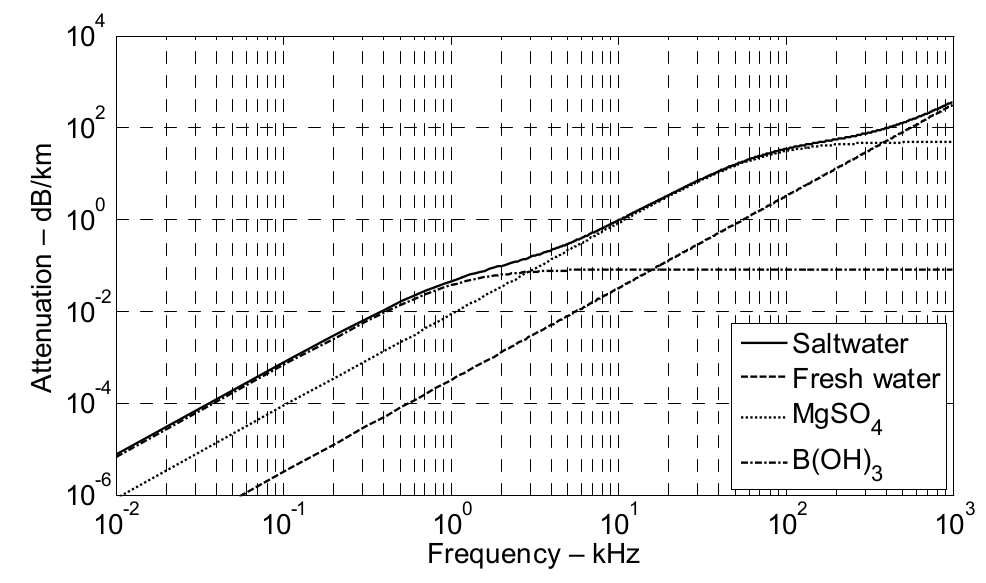
\includegraphics[scale=1.4]{waterabsorption.jpeg}
    \caption{Coefficiente d'assorbimento specifico per la frequenza in varie tipologia d'acqua}
\end{figure}

Un segnale trasmesso con potenza $P$ verra' ricevuto, attenuato, con potenza $P/A(l, f)$.
\par
Per quanto riguarda il rumore da cui un segnale in acqua viene affetto, possiamo considerarlo proveniente da quattro diverse sorgenti principali:
\begin{itemize}
    \item Turbolenza in acqua: $10log\ N_t(f) = 17 - 30log\ f$
    \item Navi di passaggio: $10log\ N_s(f) = 40 + 20(s - 0.5) + 26log\ f - 60log\ (f+0.03)$
    \item Onde: $50 + 7.5w^{1/2}+ 20logf - 40log\ (f+0.4)$
    \item Rumore termico: $-15 + 20logf$
\end{itemize}
Come vediamo, le intensita' delle diverse sorgenti di rumore dipendono, ciascuna in maniera diversa, dalla frequenza del rumore e inficiano dunque su spettri di frequenze differenti. La turbolenza del movimento dell'acqua ha effetto a frequenze molto basse, mentre il rumore generato dal passaggio di navi e' da considerarsi non trascurabile fra i 10 ed i 100 $Hz$ (dipende anche da un fattore di "attivita' navale" $s$, compreso fra 0 ed 1). Il rumore generato dalle onde e' predominante nel range di frequenze tra i 100 $Hz$ e i 100 $kHz$, mentre quello termico lo diviene oltre i 100 $kHz$.
\begin{figure}[H]
    \centering
    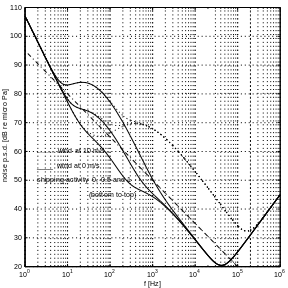
\includegraphics[]{noise.png}
    \caption{Densita' di potenza del rumore totale rispetto alla frequenza}
\end{figure}
Come si nota chiaramente dal grafico, il rumore diminuisce con l'aumentare della frequenza, fornendo cosi' una sorta di limite inferiore alla banda di frequenze da utilizzare per la trasmissione.
\par
Avendo ora descritto sia l'attenuazione del segnale sia il rumore che incide su di esso, possiamo in ultimo valutare il rapporto segnale/rumore di un segnale acustico in acqua (Signal-to-noise-ratio, SNR).
Sia $P$ la potenza di trasmissione del segnale, avremo:
\[SNR(l, f) = \frac{P/A(l, f)}{N(f)\Delta f}\]
dove $\Delta f $ e' una piccola banda di frequenze intorno ad $f$. Il fattore $1/A(l, f)N(f)$ ci indica l'andamento del SNR. Fissando la distanza di trasmissione $l$, per ciascuno di questi valori otteniamo uno specifico andamente dell'SNR in base alla frequenza $f$. Come vediamo, per ciascuna distanza esiste una specifica frequenza $f_0(l)$ per la quale il valore di $1/A(l, f)N(f)$ (e quindi dell'SNR) e' massimo.
\begin{figure}[H]
\centering
    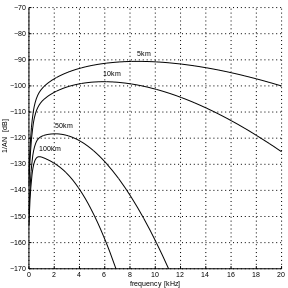
\includegraphics[]{snr.png}
    \caption{Andamento di 1/AN (SNR) rispetto alla frequenza per varie distanza considerate}
\end{figure}

La frequenza ottimale $f_0$ diminuisce con l'aumentare della distanza della trasmissione.
\begin{figure}[H]
    \centering
    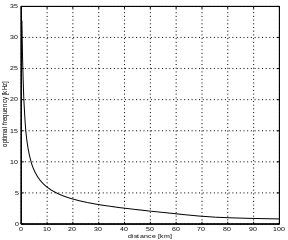
\includegraphics[]{optimalfreq.png}
    \caption{Frequenza ottimale di funzionamento rispetto alla distanza della comunicazione}
\end{figure}
\par
Nell'ambiente simulativo di cui ci si e' serviti per testare il protocollo sviluppato, il canale di comunicazione acustico e le caratteristiche appena descritte vengono rese rifacendosi al modello di Urick \cite{urick}, che fornisce una serie di formule empiriche per modellare al meglio il canale di trasmissione.

\subsection{Modelli di architetture di UWSNs}
In questo paragrafo vengono brevemente presentate tre possibili architetture per le reti di sensori sottomarini \cite{underwater}. L'architettura e la topologia di rete risultano fondamentali nel determinare fattori quali il consumo energetico complessivo della rete, la sua capacita' di trasporto e la sua affidabilita'. \newline Come anticipato, vengono qui prese in esame tre tipi di rete, che si differenziano sia per quanto riguarda la tipologia di nodi impiegati sia la loro diposizione nello spazio.  La prima di queste e' una tipologia di rete con una topologia bidimensionale composta solamente da nodi fissi ancorati al fondale marino.

\begin{figure}[H]
    \centering
	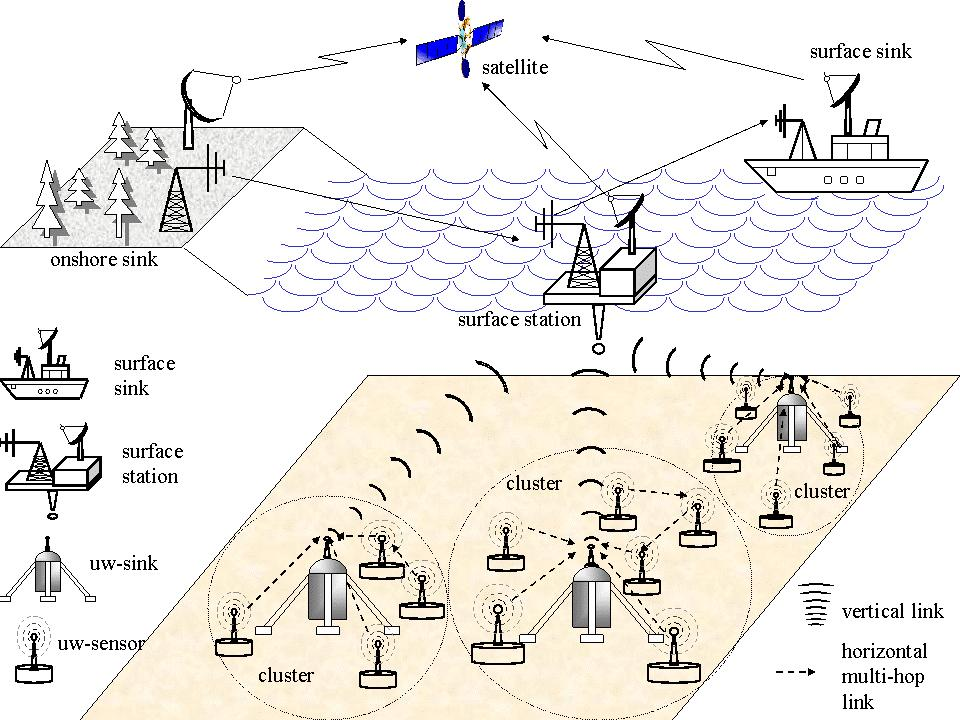
\includegraphics[scale=0.3]{2D_arch.jpg}
	\caption{ Topologia nodi fissi 2D}
	\label{fig:}
\end{figure}

Questi sensori, dotati di modem acustici, sono connessi a degli underwater sinks (uw-sinks nella figura). Questi ultimi svolgono la funzione di ``collettori'' dei dati trasmessi dai sensori, instradandoli verso la superficie marina dove vengono raccolti da una stazione ivi posta. Da notare come gli uw-sinks debbano essere dotati di due modem acustici, uno per le trasmissioni orizzontali con i sensori posizionati sul fondale ed uno per le trasmissioni verticali con la stazione di superficie (quest'ultimo e' spesso un modem per trasmissioni a lungo raggio, vista la profondita operazionale dell'uw-sink). La stazione di superficie comunica contemporaneamente con diversi uw-sink e puo' trasmettere i dati ricevuti direttamente a terra, ad una nave d'appoggio o ad un satellite.
In questo tipo di reti, spesso capita che un sensore non si trovi in prossimita' di un uw-sink ergo la comunicazione diretta con quest'ultimo sarebbe pesantemente inficiata dall'attenuazione dovuta all'elevato range di trasmissione. Una soluzione solitamente adottata in questi casi consiste nel far svolgere ai sensori anche la funzione di routing, consentendo percorsi multi-hop da un sensore verso l'uw-sink di riferimento (cio' ovviamente aumenta la complessita' del protocollo di trasmissione dei dati e dell'elaborazione di ciascun sensore).

La seconda tipologia di rete analizzata consiste ancora di soli sensori fissi, ma questa volta organizzati in uno spazio tridimensionale.

\begin{figure}[H]
    \centering
	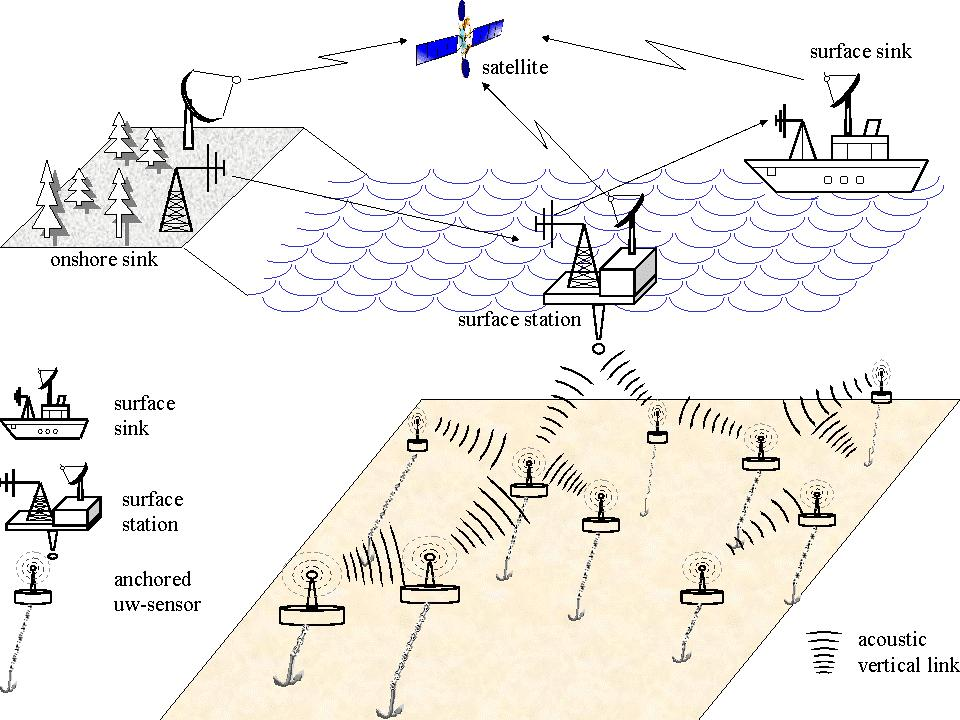
\includegraphics[scale=0.3]{3D_arch.jpg}
	\caption{ Topologia nodi fissi 3D}
	\label{fig:}
\end{figure}

In questo caso i sensori debbono svolgere una funzione che richiede loro di disporsi a diverse profondita'. Per effettuare il posizionamento, e' possibile agganciare i sensori a delle boe galleggianti (che pero' risultano visibili in superficie e possono essere d'intralcio alla navigazione) oppure e' possibile agganciare direttamente il sensore ad una boa ed ancorare la stessa, tramite una corda, al fondo marino.  In questo modo e' possibile regolare dinamicamente la profondita' del sensore tramite motore elettrico in grado di allungare/accorciare la corda d'ancoraggio. Come evidente dall'immagine, in questa topologia manca del tutto il concetto di uw-sink. I sensori sono costretti a comunicare con la stazione di superficie in modalita' multi-hop e quindi debbono necessariamente implementare le funzionalita' tipiche di un router, con l'onere computazionale aggiuntivo che cio'comporta. A causa delle correnti marine, spesso i nodi di questa tipologia di reti subiscono modifiche non volute al proprio posizionamento. Diventa quindi fondamentale la comunicazione e la collaborazione fra i sensori di questa rete in modo che ciascuno di essi possa riconfigurare in corso d'opera la propria profondita', in funzione di due obbiettivi primari:
\begin{itemize}

 \item Mantenere la copertura totale nel rilevamento della colonna interessata dalla raccolta dati dei sensori

\item Mantenere la connessione della topologia di rete, ovvero far si che esista, per ciascun nodo, un percorso fruibile verso la stazione di superficie
\end{itemize}

La terza e ultima topologia di rete presa in considerazione espande le caratteristiche delle prime due configurazione analizzate introducendo la presenza di nodi mobili all'interno della rete (Autonomous Underwater Vehicle, AUV).

\begin{figure}[h]
	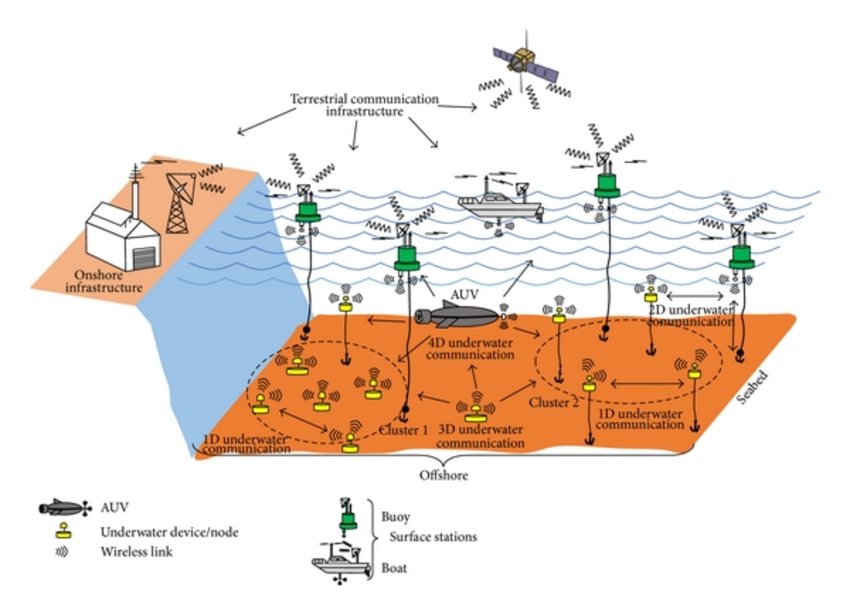
\includegraphics[width=\linewidth]{auv_arch.png}
	\caption{ Topologia comprendente nodi mobili}
	\label{fig:}
\end{figure}

L'introduzione di nodi mobili all'interno della rete espande enormemente le capacita' di una UWSN, dato anche il costo relativamente basso di un AUV equipaggiato con diversi sensori. La presenza di nodi mobili nella rete permette, ad esempio, l'adaptive sampling, ovvero la possibilita' di posizionare adattativamente i sensori mobili presso un particolare punto d'interesse, variando la densita' di sensori presenti in quella data zona. Inoltre, facendo riferimento alle questioni sorte nella trattazione della rete tridimensionale di nodi fissi, appare chiaro come un AUV possa, data la sua maggior liberta' di movimento, ovviare facilmente a deficit nella copertura di un area o ad eventuali buchi che si vengono a creare nella rete (ad esempio andando a sostituire un nodo fisso malfunzionante andando a posizionarsi in prossimita' di questo).
Esistono in commercio diversi tipi di AUV, fra i quali ricordiamo:
\begin{itemize}

\item i drifters, ovvero veicoli che viaggiano seguendo la corrente oceanica in cui sono immersi, con la possibilita' di variare solamente la propria
profondita d'azione

\item i gliders (``alianti''), dotati di timone di coda e di ali laterali, i quali possono variare la propria linea di galleggiamento in modo da alimentare la propria spinta propulsiva in avanzamento

\item AUV simili a veri e propri sottomarini in miniatura, dotati di propulsione elettrica tramite eliche

\end{itemize}
\begin{figure}[H]
    \centering
	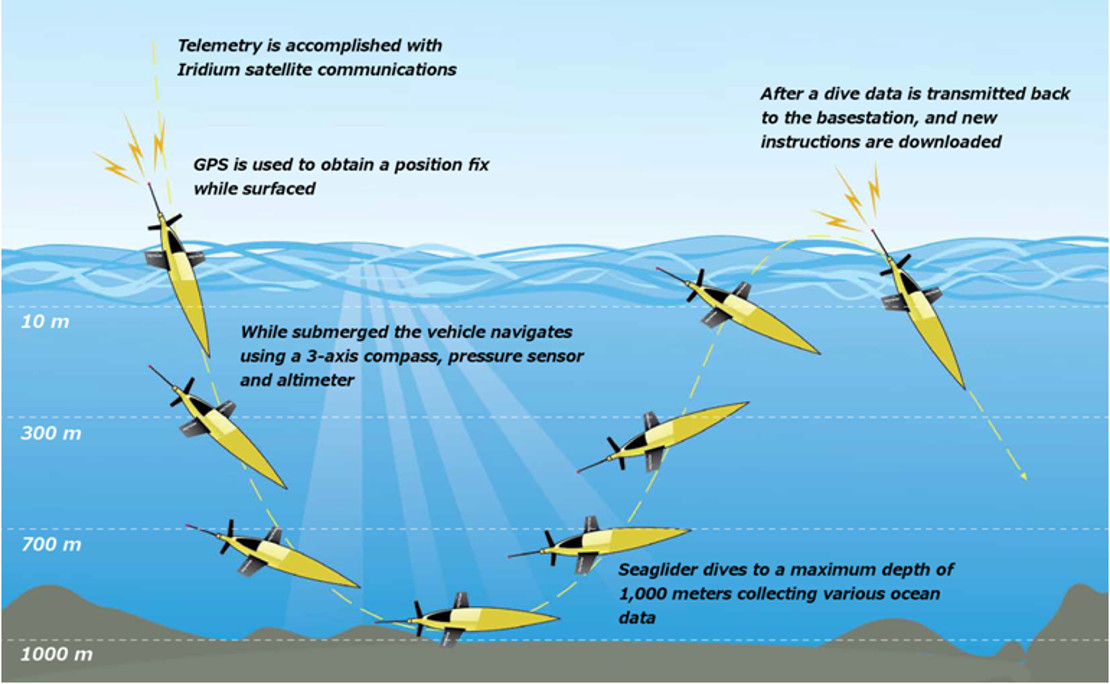
\includegraphics[width=\linewidth]{glider.jpg}
	\caption{ Esempio di funzioamento di un glider}
	\label{fig:}
\end{figure}


\begin{figure}[H]
    \centering
	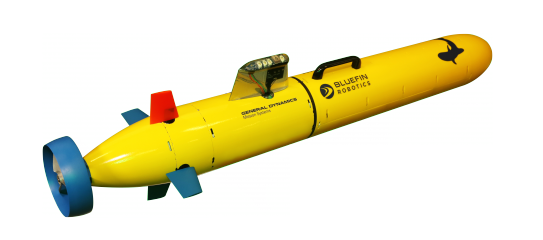
\includegraphics[width=\linewidth]{auv.png}
	\caption{ Esempio di AUV}
	\label{fig:}
\end{figure}

\subsection{SUNSET: Sapienza Underwater }

SUNSET, acronimo di Sapienza Underwater Networking framework for underwater Simulation and Emulation and real-life Testing, e' un framework per lo sviluppo ed il testing di protocolli per reti underwater ed e' stato scelto come ambiente di sviluppo e valutazione del protocollo di localizzazione ivi analizzato \cite{sunset}.\newline
SUNSET e' basato sul simulatore di reti open-source ns-2 e su una sua estensione, ns2-Miracle, ampiamente utilizzati in quest'ambito scientifico, il che permette agli sviluppatori gia' usi a questi strumenti una rapida transizione verso l'utilizzo di questo framework.
SUNSET prevede tre modalita' di utilizzo: simulation, emulation e real-life testing.
La prima permette di simulare preventivamente il funzionamento della rete, in maniera totalmente indipendente dall'hardware che verra' utilizzato nel test reale, fornendo agli sviluppatori la possibilita' di testare le proprie soluzioni protocollari in un ambiente controllato variando una moltitudine di parametri ambientali e di configurazioni. Fra queste, ricordiamo le diverse soluzioni per quanto concerne il modello di trasmissione dei segnali acustici in acqua: formule empiriche ( come il modello di Urick), il simulatore di propagazione Bellhop (incluso tramite WOSS) e dati reali del canale replicabili all'interno del simulatore.
\newline
Una delle caratteristiche peculiari che rendono SUNSET una soluzione d'avanguardia nel settore consiste nel rendere praticamente immediato il passaggio dall'ambiente simulativo a quello emulativo/real-life. Difatti, al costo di lievi modifiche al codice sorgente, i protocolli sviluppati possono essere impiegati indipendentemente sia nella modalita' di simulazione che nelle altre due modalita'. Questa caratteristica garantisce a SUNSET un enorme vantaggio rispetto ad altre soluzioni software operanti nello stesso ambito. Basti pensare al costo, in termini di tempo e denaro, del testing reale di una nuova tecnologia in ambito di UWSNs, comprendente come voce non trascurabile la traduzione delle tecnologie sperimentate nell'ambiente simulativo in strumenti operativi concretamente fruibili. SUNSET rende praticamente trascurabile lo sforzo da parte degli sviluppatori per questa operazione.
\newline
Nello sviluppo di SUNSET si e' voluta separare la componente riguardante l'implementazione della pila protocollare dai moduli utili al controllo della componentistica reale in modalita' di emulazione. Pertanto, lo sviluppatore puo' modificare, ad esempio, la logica di funzionamento di un protocollo senza intaccare in alcun modo i driver di controllo dei vari device e viceversa.
Una novita' introdotta nell'ultima versione di SUNSET, identificata' dal termine "backseat-driver", ha come scopo dare maniera agli sviluppatori di modificare, in real-time durante lo svolgimento di un test sul campo, la configurazione di una rete di sensori underwater gestita tramite SUNSET. Si puo', ad esempio, modificare la topologia di rete, spegnendo od accendendo dei nodi, oppure mutare i parametri di funzionamento di un protocollo.
\newline
SUNSET supporta in maniera ottimale ben 5 modem acustici in circolazione, oltre a numerosi sensori disponibili in commercio, offrendo una piattaforma unitaria sia per il controllo delle funzionalita' di rete sia per il data sensing. Non ultima l'efficienza in termini di costo computazionale, che permette a SUNSET si essere eseguito su piattaforme dotate di risorse di calcolo limitate (ad esempio Gumstix ed altri sistemi ARM-based).


\section{Sistemi di localizzazione acustica sottomarini}
Appare chiaro come, sia per sensori fissi che per AUVs, i dati da essi raccolti abbiano molto spesso valore solamente se integrati dall'informazione circa la posizione esatta nella quale gli stessi sono stati rilevati. Inoltre alcuni servizi, quali ad esempio la copertura di zone d'ombra che dinamicamente si vengono a creare in una rete, non sarebbero possibili senza una precisa localizzazione degli elementi stessi della rete.
Vediamo in breve le principali tecniche di localizzazione esistenti.

\subsection{Tecniche di localizzazione}
Per localizzazione intendiamo quella procedura atta a determinare la posizione di un sensore, fisso o mobile, in termini di coordinate spaziali. Le coordinate possono riferirsi ad un sistema di riferimento globale (es. latitudine, longitudine e profondita') oppure relative ad un sistema di coordinate locali (come ad esempio coordinate relative ad un particolare sensore preso come origine di un sistema di riferimento cartesiano).
\par
Per qualunque sistema di localizzazione, due paramentri sono fondamentali per valutarne l'affidabilita':
\begin{itemize}
    \item Accuratezza: quanto la posizione calcolata sia distante dalla posizione reale
    \item Precisione: quanto le misurazioni effettuate siano fra loro consistenti
\end{itemize}
Ad esempio, un sistema di localizzazione con accuratezza 3$m$  e precisione dell'80\% delle misurazioni ci rassicura sul fatto che 8 volte su 10 la posizione che esso calcolera' sara' errata di al piu' 10$m$.
\par
Nei sistemi di localizzazione, le misure principali richieste per effettuare i calcoli necessari sono delle distanze relative. Queste sono calcolabili utilizzando il ToA, Time-of-Arrival, ovvero il tempo di propagazione richiesto ad un segnale per compiere il tragitto da un emettitore ad un ricevente. Conoscendo la velocita' di propagazione del segnale nel mezzo specifico, possiamo calcolare la distanza fra sorgente e destinatario del segnale.
Possiamo categorizzare i sistemi di localizzazione in alcune classi principali \cite{trilateration}:
\begin{itemize}
    \item One-way ToA: la distanza viene calcolata utilizzando la propagazione di un solo segnale (e richiedono percio' elevata sincronizzazione temporale tra i due nodi):
    \[dist_{ij}\ =\ (t_2-t_1)*v\]
    \item Two-way ToA: la distanza viene calcolata misurando il RTT di un segnale e non richiede sincronizzazione tra i nodi:
    \[dist_{ij}\ =\ \frac{(t_4-t_1)-(t_3-t_2)}{2}*v\]
    \item Time Difference of Arrival (TDoA): due segnali con differenti velocita', il primo di velocita' $v_1$ inviato all'istante $t_1$ e ricevuto a $t_2$ e l'altro di velocita' $v_2$ inviato a $t_3 = t_1 + t_{wait}$ e ricevuto a $t_4$. Non si richiede sincronizzazione tra i due nodi, ma c'e' la necessita' di due sorgenti differenti di segnale.
    \[dist = (v_1 - v_2)*(t_4 - t_2 - t_wait)\]
    \item Angle of Arrival (AoA): sistema che richiede un array di antenne o microfoni. La ricezione dello stesso segnale da ciascun ricevitore con caratteristiche differenti (tempo d'arrivo, fase, ampiezza) consente di calcolare l'angolo fra il segnale ed un certo punto di riferimento, oltre alla distanza.
    \item Received Signal Strength (RSS): sistemi in cui il calcolo della distanza dall'emettitore del segnale avviene conoscendo la potenza iniziale del segnale, quella con cui lo si e' ricevuto e il modello che descrive il decadimento del segnale con la propagazione.
\end{itemize}
Il sistema USBL, di cui parleremo subito dopo, appartiene alla categoria di sistemi di localizzazione AoA, mentre quelli SBL e LBL sono di tipo Two-way ToA o Onw-way ToA.
Questi ultime due classi di sistemi fanno ricorso, per il calcolo effettivo della posizione, al metodo matematico della trilaterazione.
Conoscendo la distanza dell'oggetto da localizzare rispetto ad un nodo fisso, l'oggetto deve necessariamente giacere sulla superficie di una sfera (in due dimensioni, sul perimetro di una circonferenza) centrata nel nodo fisso ed avente raggio pari alla distanza calcolata. Possiamo quindi impostare un sistema di tante equazioni di secondo grado (equazione della superficie di una sfera) quanti sono i nodi fissi da cui conosciamo la distanza. Risolvendo il sistema (con tecniche di cui parleremo nella parte dedicata al protocollo sviluppato) si puo' ottenere la posizione dell'oggetto d'interesse.

\subsection{LBL, USBL, SBL}
I sistemi acustici di localizzazione sottomarina possono essere classificati in tre categorie, in base al principio di funzionamento utilizzato ed alla modalita' con cui viene approntato il sistema. \cite{underwaterpositioning} \newline
In primis, consideriamo i sistemi LBL (Long-baseline).  Il loro funzionamento dipende dal posizionamento di 3 o piu' transponders vengano piazzati sul fondale marino (o ad una certa altezza dal fondale), la cui posizione deve essere nota in maniera precisa. 
I transponders vengono posti solitamente al margine dell'area operativa dei veicoli che si intende localizzare, ad una distanza abbastanza elevata ciascuno dall'altro. Sul nodo mobile viene montato un segnalatore che invia un segnale acustico ai transponders. Questi ultimi ricevono il segnale e lo reinviano al veicolo. Tramite il time-of-flight del segnale, il veicolo conosce la propria distanza da ciascuno dei transponders e puo' effettuare la localizzazione (ad esempio tramite triangolazione o trilaterazione).

\begin{figure}[H]
    \centering
	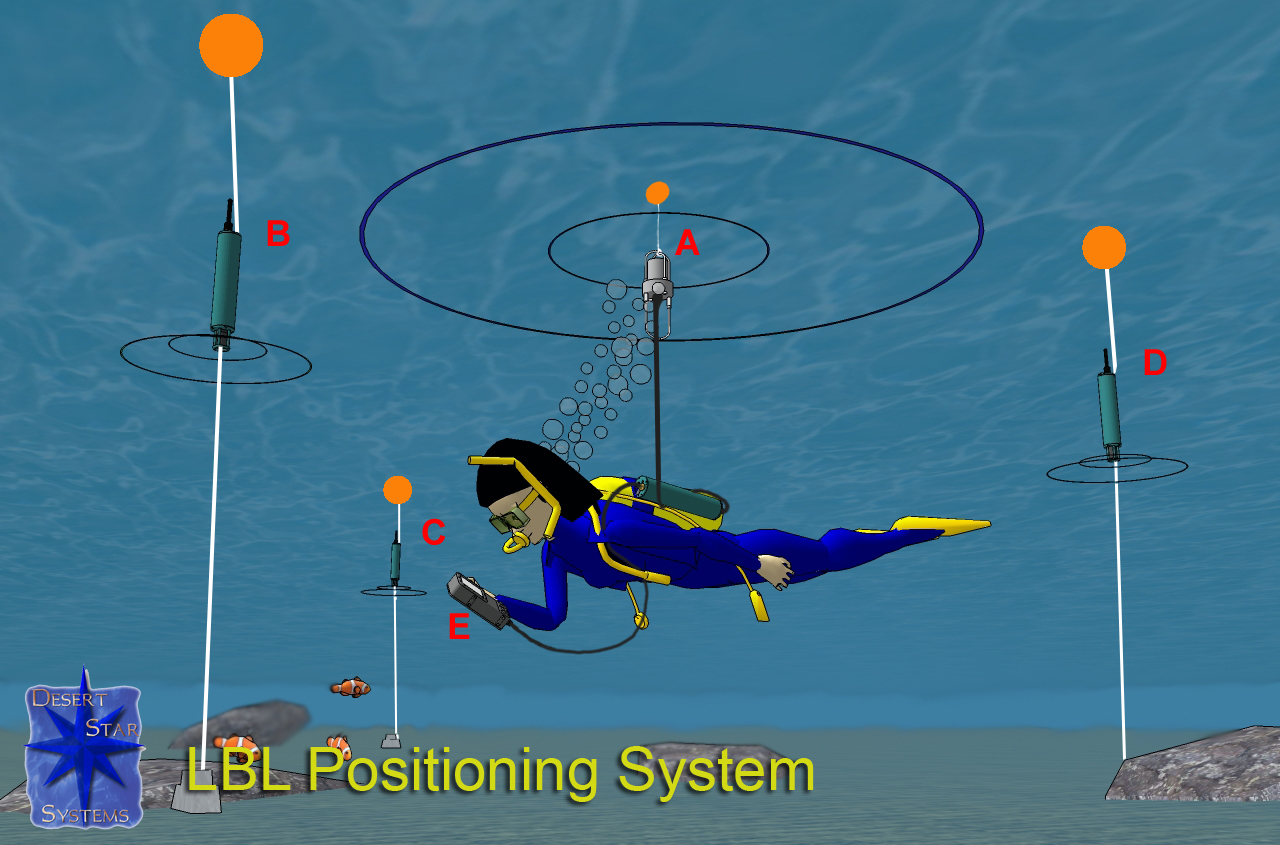
\includegraphics[scale=0.25]{LBL.jpg}
	\caption{ Esempio di localizzazione LBL}
	\label{fig:LBL}
\end{figure}
\newpage

I sistemi USBL (Ultra Short Base-line ) sfruttano invece un'array di trasduttori, montati solitamente sul fondo di una barca. L'AUV invia un segnale che viene ricevuto da questi trasduttori i quali, dal time-of-flight, calcolano la distanza del nodo mobile dall'imbarcazione e, utilizzando la differenza di fase fra il segnale ricevuto dai diversi trasduttori, ne calcolano anche la direzione. Dalla combinazione di distanza e direzione si ottiene la posizione dell'AUV, che pero' risulta notevolmente meno precisa di quella ottenuta con metodo LBL ( ma richiede un segnale in meno). L'errore nel posizionamento dipende fondamentalmente dalle imprecisioni nella direzione calcolata (in particolare quando l'AUV e' lontano dai trasduttori).\newline
In ultimo , i sistemi SBL (Short Base-line), simile a quelli USBL per la mancanza di transponders fissati al fondale ma che sfruttano un meccanismo simile a quello degli LBL. Infatti, in questi sistemi, 3 o piu' transponders vengono collegati ad un sistema di controllo centrale ed immersi in acqua, solitamente attaccati sul fondo di una barca o di un molo. Uno di questi transponders invia un segnale che viene ricevuto dal nodo mobile, che a sua volta risponde inviando un segnale a tutti i transponders. Dai tempi di propagazione viene ricavata la distanza dell'AUV , utilizzata poi nel calcolo della localizzazione come nel caso dei sistemi LBL.

\begin{figure}[H]
	\centering
	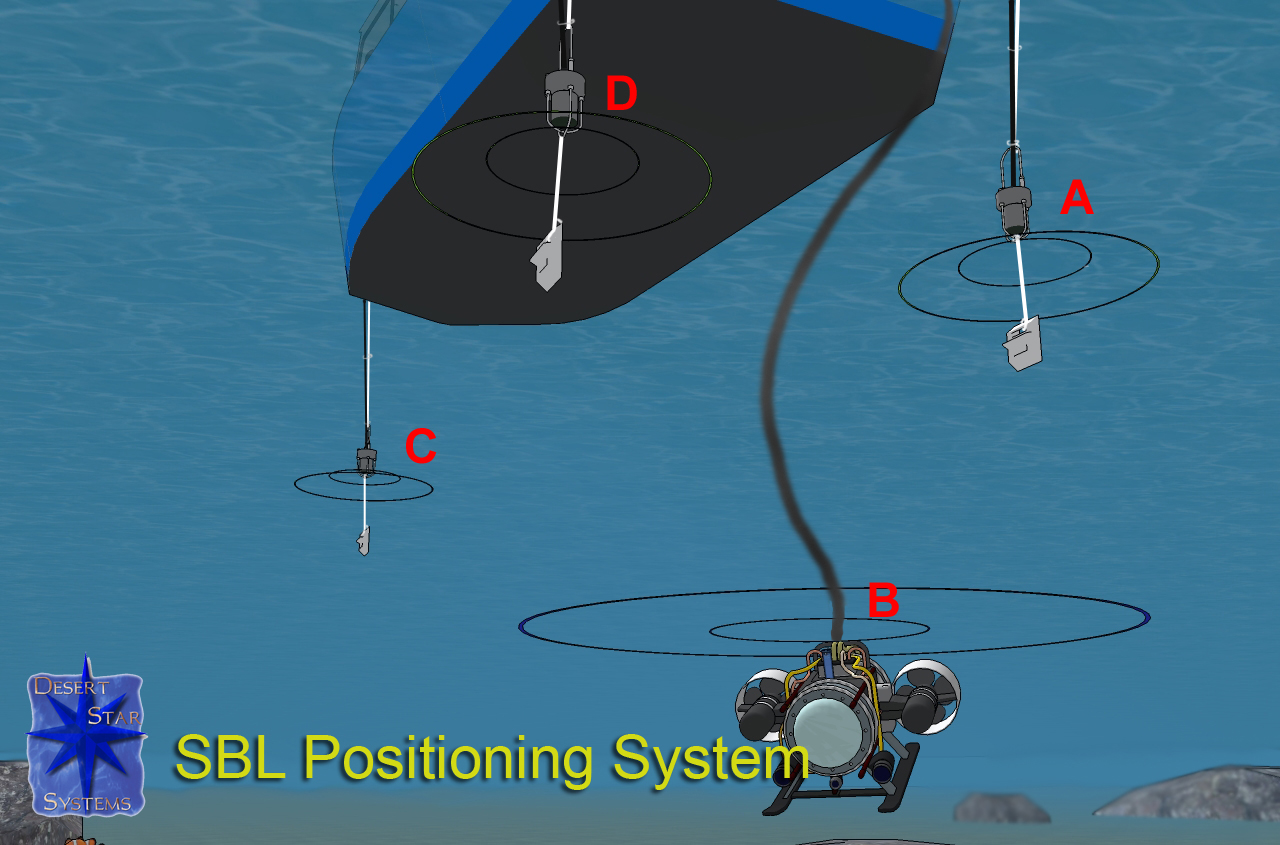
\includegraphics[scale=0.25]{SBL.jpg}
	\caption{ Esempio di localizzazione SBL}
	\label{fig:SBL}
\end{figure}


\par
In quest'elaborato si e' scelto di replicare un sistema di localizzazione sul modello di quelli LBL. Nel nostro caso, al posto dei transponders, vengono utilizzati dei nodi fissi (intesi come sensori fissati o agganciati al suolo) e non vengono scambiati dei semplici e brevi segnali acustici ma dei veri e propri pacchetti di rete. In questo modo, la localizzazione di un nodo mobile avviene contemporaneamente allo scambio di informazioni di altro tipo (ad esempio comandi di riconfigurazione inviati dall'AUV ai nodi fissi o dati raccolti dai nodi fissi all'AUV), al costo della sola aggiunta di un nuovo header ai pacchetti trasmessi.  


\chapter{MARTA e il suo modello di mobilita'}

\section{MARTA}

MARTA (MARine Tool for Architecture) e' un AUV sviluppato dall'Universita' di Firenze nell'ambito dell'iniziativa ARROWS, progetto supportato dalla Commissione Europea che aveva come obbiettivo lo sviluppo di tecnologie a basso costo da mettere a disposizione degli archeologi impegnati in ricerche in ambienti sottomarini. In quest'ottica, MARTA viene pensato come veicolo impiegabile in ruoli di ricerca di punti d'interesse all'interno dell'area archeologica e della loro successiva ispezione (acquisizione di immagini del punto individuato). \newline
Questo risultato viene raggiunto grazie alla natura modulare del progetto di questo AUV, che garantisce un'elevata personalizzabilita' della configurazione operativa del veicolo ( a livello di payload di sensori ottici/acustici, tipo di propulsione, power source). \newline
Inoltre, MARTA viene equipaggiato con due modem acustici, diversi per velocita' di trasmissione/consumo energetico, il che lo rendono adatto a svolgere il ruolo di "ponte" comunicativo per i dispositivi BR (Biometric Robots), solitamenti impegnati ad analizzare le zone piu' difficilmente accessibili dell'area archeologica subacquea.

\begin{figure}[H]
	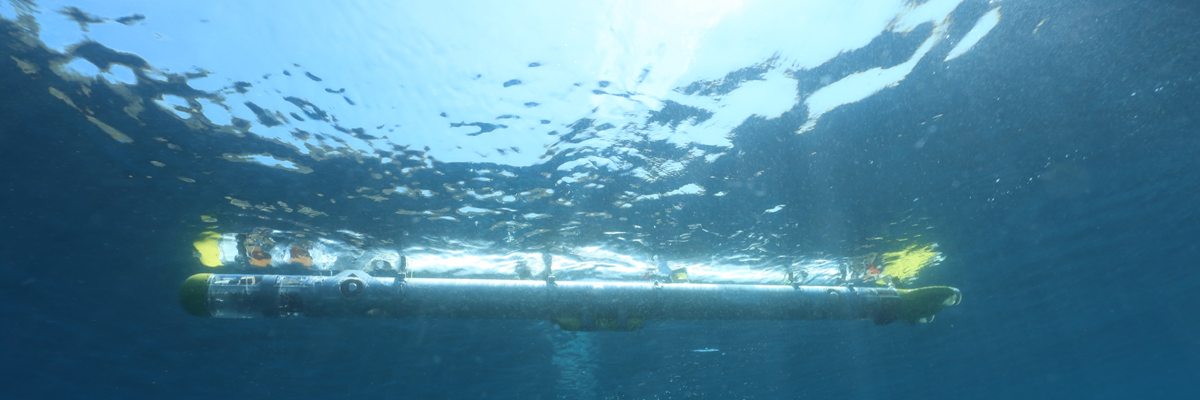
\includegraphics[width=\linewidth]{MARTA.png}
	\caption{MARTA in superficie}
	\label{fig:MARTA}
	\centering
\end{figure}

Per quanto riguarda le dimensioni del veicolo, MARTA ha una lunghezza massima di 3.7 $m$ (nella sua configurazione completa), pesa 80 $kg$ fuori dall'acqua ed  ha un diametro esterno di 180 $mm$. Il movimento del veicolo e' vincolato a 5 gradi di liberta'. Infatti MARTA puo' muoversi in verticale, salendo o scendendo di profondita', ruotare mantenendosi parallelo al piano orizzontale e spostarsi in avanti nella direzione stessa del veicolo, oltre a poter stazionare fisso in punto. La mobilita' del veicolo e' controllata da 6 attuatori, di cui 2 eliche posteriori, 2 eliche laterali e 2 eliche verticali. Il veicolo puo' raggiungere una profondita' massima di 120 $m$, viaggiando tipicamente ad una velocita' media di 1 nodo al secondo ( la velocita' massima dichiarata e' di 3 nodi al secondo). \newline 
Il controllo del veicolo e' affidata al software ROS (Robot Operating System), che presenta un architettura altamente modulare che ben si adatta alla modularita' del design progettuale di MARTA.

\subsection{Implementazione modello di mobilita' di MARTA su SUNSET}
Le specifiche caratteristiche di mobilita' di MARTA hanno richiesto la necessita' di intervenire sulla gestione della simulazione del movimento di un nodo all'interno del framework SUNSET. \newline In particolare, MARTA presenta due vincoli di movimento cui prestare attenzione. In primis, il veicolo in questione non puo' contemporaneamente muoversi in avanti e variare la sua quota di profondita', essendo le due modalita' di spostamento mutuamente esclusive. In secondo luogo, MARTA puo' variare la propria direzione di spostamento sul piano orizzontale solamente in posizione stazionaria, ergo qualunque cambio di direzione richiede preventivamente che il veicolo si fermi e solo in seguito effettui la rotazione necessaria, utilizzando le eliche laterali.\par
Dati quindi dei generici waypoints, rappresentanti il percorso di un AUV, si e' voluto, all'interno di SUNSET, far si che il simulatore generasse un nuovo insieme di waypoints che includesse l'insieme originario e generasse un nuovo percorso conforme ai vincoli di movimento introdotti da MARTA. \newline Per far ottenere questo risultato, e' stata creata una specifica funzione in linguaggio Tcl.  All'interno di questa vengono iterativamente prese in esame i waypoints passati in input allo script simulativo (salvati all'interno di un apposita variabile globale). Per ciascuna posizione, viene considerata la posizione precedente da cui l'AUV proviene. Se quest'ultima si trova ad una profondita' differente dalla posizione in esame, la funzione aggiunge al percorso dell'AUV un waypoint intermedio, avente come coordinate geografiche proprio quelle del waypoint precedente a quello analizzato ma sito alla stessa profondita' del nodo in esame, dimodoche' il movimento del veicolo avvenga prima lungo la verticale e poi in orizzontale, in maniera consona al modello di movimento di MARTA.\newline
Nella figura sottostante, si consideri il punto B come il waypoint in esame in una specifica iterazione, il punto C la posizione successiva da raggiungere ed il punto A la posizione precedentemente attraversata.\newline L'angolo $\varphi$  e' quindi l'angolo di cui e' necessario ruotare l'AUV prima di dirigersi verso il nodo C, una volta raggiunto il punto B (indipendentemente dal fatto che il nodo C si trovi ad una quota differente rispetto a B). 

\begin{figure}[H]
    \centering
	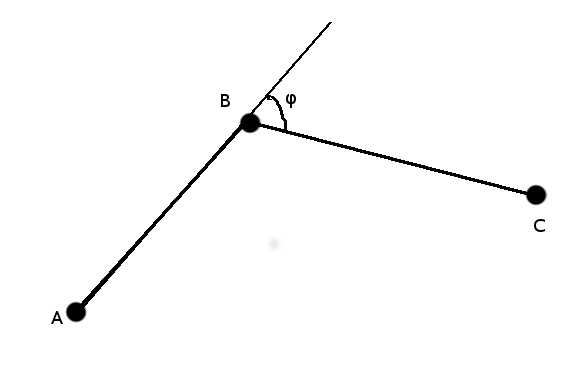
\includegraphics[scale=0.5]{scalarprod.png}
\end{figure}

Per calcolare quest'angolo, si ricorre semplicemente alla formula del prodotto scalare fra due vettori, in questo caso i vettori AB e BC, ottenuti dalla conoscenza delle coordinate geografiche dei rispettivi waypoints (previa trasformazione in coordinate cartesiane nel sistema ECEF, Earth Centered Earth Fixed ). Per la formula del prodotto scalare:


\begin{equation}
\overrightarrow{AB} \cdot \overrightarrow{BC} = |AB| |BC| \cos{\varphi}    
\end{equation}

 
Si ottiene cosi' il valore dell'angolo $\varphi$ che, diviso per la velocita' di rotazione dell'AUV, da' la misura del tempo di rotazione impiegato da MARTA per effettuare il cambio di direzione. \newline L'intervallo temporale cosi' calcolato viene passato in input alla funzione di aggiunta del waypoint corrispondente alla posizione B.
 Difatti il sistema di gestione dei waypoints consente di specificare, contestualmente alla creazione del putno, un tempo nel quale l'AUV e' costretto a sostare fermo nella posizione del waypoint prima di riprendere il suo percorso. In questo modo, il tempo di rotazione richiesto da MARTA viene trasformato in questo tempo d'attesa, ottenendo come risultato finale un modello di movimento del tutto rispondente ai vincoli imposti dal veicolo in considerazione.\newline
Queste trasformazioni sono state applicate ad un percorso "a serpentina", tipico per missioni di perlustrazione/monitoraggio di una certa area marina dai confini ben definiti. Riportiamo in basso i grafici del percorso dell'AUV non modificato e quello ottenuto imponendo i vincoli di movimento di MARTA.

\begin{figure}[h!]
	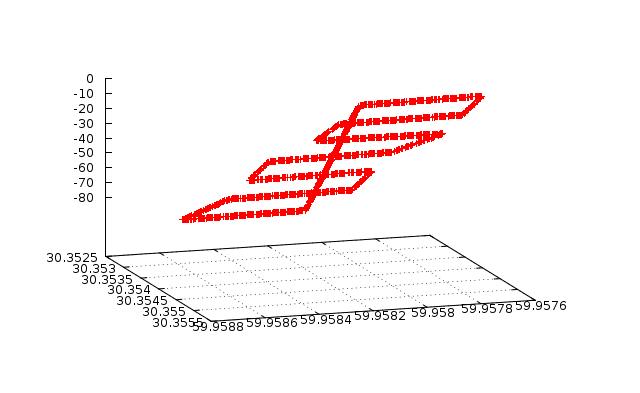
\includegraphics[width=\linewidth]{posizioninoscript.png}
	\caption{Percorso dell'AUV senza vincoli}
	\label{fig:}
	\centering
\end{figure}

\begin{figure}[h!]
	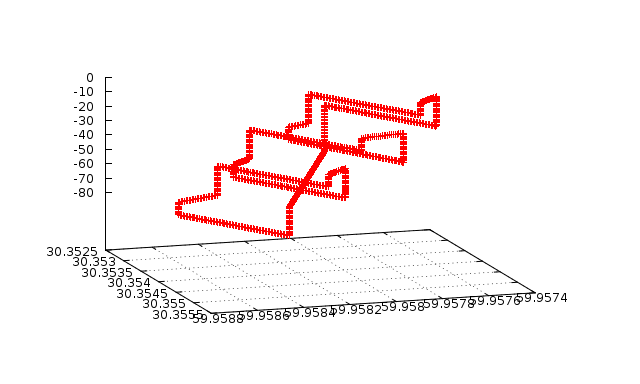
\includegraphics[width=\linewidth]{posizioniscript.png}
	\caption{Percorso dell'AUV con vincoli}
	\label{fig:}
	\centering
\end{figure}



\chapter{Protocollo di localizzazione}

\section{Descrizione del protocollo}
Il protocollo di localizzazione realizzato rientra nella categoria dei protocolli di localizzazione "a due vie" (Two-Ways Ranging Protocols), nello specifico alla categoria dei sistemi di posizionamento LBL (vedi par. 1.2.1).\newline Difatti il funzionamento del protocollo richiede che il nodo mobile, di cui si vuole conoscere la posizione, effettui una richiesta di localizzazione in modalita' broadcast. I nodi fissi della topologia, ricevuta la richiesta, rispondono ciascuno in modalita' "unicast" al nodo mobile (data la natura del mezzo trasmissivo, le risposte vengono ovviamente ricevute da molti nodi presenti nella topologia, ma vengono scartate discernendo rispetto al destinatario della risposta).  Una volta collezionate un minimo di 3 riposte, il nodo mobile, conoscendo a priori la posizione dei nodi fissi e potendo calcolare la propria distanza da ciascuno di essi attraverso i dati contenuti nell'header delle risposte ricevute, puo' cosi' calcolare la propria posizione tramite triangolazione, in maniera del tutto simile al funzionamento di un localizzatore GPS.

A livello dello stack dei protocolli di rete, il protocollo di localizzazione si inserisce al livello MAC, posto direttamente sopra il protocollo di livello fisico. Data la possibilita' fornita da SUNSET di far collaborare diversi protocolli per uno stesso livello dello stack protocollare, e' possibile affiancare il protocollo di localizzazione a protocolli MAC veri e propri (es. Slotted Aloha). Il protocollo di localizzazione, nel caso l'AUV richieda di calcolare la propria posizione, non fa altro che aggiungere un header al pacchetto in maniera trasparente al resto della pila protocollare.

\subsection{Esempio di funzionamento}
Viene qui descritto un esempio del funzionamento del protocollo sopra descritto.\newline Il nodo mobile, mentre e' in movimento, invia una richiesta di localizzazione, settando come indirizzo sorgente il proprio codice identificativo all'interno della topologia (tipicamente un intero univoco per ciascun nodo)
ed inserendo come indirizzo di destinazione l'indirizzo di broadcast.\newline L'AUV continuera' a muoversi mentre aspetta di ricevere le risposte dei nodi fissi. Da notare che l`AUV collezionera' solamente le risposte pervenute entro un certo intervallo di tempo dal momento di invio della richiesta (il valore di questo intervallo temporale verra' discusso nel capitolo successivo).\newline
Questi ultimi, non appena ricevuta la richiesta di localizzazione, creano il pacchetto di risposta ed avviano ciascun un proprio timer. Questo timer, il cui runtime viene calcolato a partire da una distribuzione randomica uniforme (da 0 ad un valore massimo parametrizzato), adempie al compito di desincronizzare le risposte dei nodi fissi,
facendo in modo che si verifichino un minor numero di collisioni fra i pacchetti (essendo il mezzo condiviso).\newline Da notare, come gia' detto, che la risposta viene inviata in modalita' "unicast", settando l'indirizzo di destinazione con quello del nodo mobile che ha generato la specifica richiesta. Potenzialmente, questo meccanismo permette la localizzazione di due o piu' nodi mobili, potendo questi ultimi discernere quali pacchetti di risposta siano a loro indirizzati da quelli diretti ad altri AUV.\newline
Ad ogni modo, l'AUV colleziona un certo numero di risposte a lui indirizzate e, una volta scaduto il timer d'attesa delle risposte, effettua i calcoli necessari alla propria localizzazione, a partire dal calcolo della propria distanza da ciascun nodo fisso da cui ha ricevuto riposta.\newline
Questo calcolo, nel caso del veicolo in movimento, viene condizionato da due tipologie d'errore che andranno ad inficiare il risultato finale della misurazione. 
In primo luogo, come gia' anticipato, l'AUV calcola la distanza dai nodi fissi a partire dal RTT. Questo valore viene moltiplicato per la velocita' del suono in acqua ( nel simulatore 1500 m/s) e il valore ottenuto viene quindi dimezzato.
Quest'ultima divisione presuppone che il tempo di propagazione della richiesta di localizzazione si pari a quello di propagazione della risposta, cosa non vera nel caso dell'AUV in movimento (si pensi al caso in cui il veicolo si stia dirigendo proprio verso un nodo fisso da cui riceve risposta).\newline
In aggiunta, la distanza viene calcolata al momento dello scadere del timer avviato dall'AUV non appena effettuata la richiesta di localizzazione e non quando il veicolo riceve la risposta.
Il valore della distanza ottenuto col calcolo sara' riferito a questo secondo istante temporale, mentre il calcolo della posizione del nodo mobile avviene al primo istante.

\subsection{Dettaglio degli headers protocollari}
Il protocollo utilizza due differenti headers, rispettivamente  per l'invio di richieste e risposte di localizzazione.
\newline
Per quanto riguarda l'header impiegato nella richiesta, esso si compone di 3 campi:
\newline

\begin{bytefield}[bitwidth=1.1em]{32}
        \bitheader{0-31} \\
            \bitbox{8}{SRC} & \bitbox{8}{DST} & \bitbox{16}{PKTID} \\
\end{bytefield}

\begin{itemize}
    \item sorgente della richiesta (SRC)
    \item destinazione della richiesta (DST)
    \item id della richiesta (PKTID)
\end{itemize}


I primi due campi contengono l'identificativo del nodo che genera la richiesta di localizzazione e l'indirizzo dei nodi a cui la richiesta e' destinata (l'indirizzo di broadcast). Il terzo campo contiene un id univoco della richiesta (necessario per la corrispondenza fra i pacchetti di risposta e la richiesta per cui sono stati generati).\par
Per quanto riguarda l'header per il pacchetto di risposta, esso contiene i seguenti campi:
\newline



\begin{bytefield}[bitwidth=1.1em]{32}
        \bitheader{0-31} \\
        \bitbox{8}{SRC} & \bitbox{8}{DST} & \bitbox{16}{PKTID} \\
            \bitbox{16}{DEFERTIME} \\
\end{bytefield}

\begin{itemize}
    \item sorgente della risposta (SRC)
    \item destinazione della risposta (DST)
    \item id della richiesta per cui e' generata la risposta (PKTID)
    \item tempo d'attesa della risposta presso il nodo fisso (DEFERTIME)
\end{itemize}
I campi SRC e DST hanno funzione analoga a quelli presenti nell'header della richiesta ma, nel caso della risposta, il campo destinazione non conterra' l'indirizzo di broadcast ma l'identificativo del nodo cui la risposta e' dedicata ( in una sorta di modalita' "unicast" ). Il campo PKTID conterra' l'id della richiesta per cui la risposta e' stata generata. In ultimo il campo DEFERTIME verra' utilizzato per salvare l'intervallo di tempo che trascorre fra l'istante in cui il nodo fisso riceve la richiesta e l'istante in cui invia la risposta.\newline
In questo modo l'AUV, una volta effettuata una richiesta di localizzazione e ricevute delle risposte dai nodi fissi, 
sapra' calcolare, per ciascuna risposta ricevuta, la propria distanza dal nodo fisso che quella risposta ha generato.\newline Per far questo, bastera' calcolare il RTT della richiesta di localizzazione,
essendo noti l'istante di invio della richiesta, il DEFERTIME dell'header di risposta  e  l'istante di ricezione della risposta. Ovviamente, per effettuare il calcolo, dovra' essere nota anche la velocita' di propagazione di un segnale acustico in acqua, valore non costante (dipendente da una serie di fattori, fra i quali temperatura', salinita' e profondita' dell'acqua). Tuttavia e' possibile dotare un AUV  di un particolare tipo di sensori chiamati CDT (Conductivity-Temperature-Depth), che misurano appunto temperatura dell'acqua, profondita' a cui si trova il sensore e la conduttivita' del mare in quel punto (da cui e' possibile ricavare la salinita'). Conoscendo  questi fattori e' possibile ricavare una stima precisa sul valore della velocita' di propagazine di un segnale acustico. 



\subsection{Parametri d'interesse e modalita' di funzionamento del protocollo}
\subsubsection{Valore massimo del timer di desincronizzazione dei nodi fissi}
Alcuni parametri fondamentali condizionano in maniera netta il funzionamento del protocollo di localizzazione.\par Uno su tutti e' l'ampiezza dell'intervallo
in cui i nodi fissi scelgono, con distribuzione uniforme di probabilita', il tempo con cui avviare il timer necessario alla desincronizzazione dei pacchetti di risposta.
Il timer serve a far si che, con ragionevole certezza, i nodi fissi rispondano ad una richiesta di localizzazione in istanti differenti l'uno dall'altro (anche nel caso ricevano la richiesta quasi nello stesso momento).
Il valore con cui viene inizializzato il timer, come detto, viene scelto a caso in un intervallo di valori che parte da 0 ad un certo valore massimo.
Ovviamente, piu' elevato sara' il valore dell'estremo superiore di questo intervallo, maggiore sara' la scelta di valori possibili per il timer, minore la possibilita' che i nodi fissi inviino riposte in istanti fra loro vicini e quindi
piu' bassa la probabilita' di collisioni fra le stesse risposte. Il maggior numero di risposte ricevute fara' si che ci sia una piu' alta percentuale di localizzazioni andate a buon fine (ricordiamo la necessita' di ricevere almento 3 risposte per effettuare il posizionamento dell'AUV).\newline
Tutto cio' a scapito della precisione nel calcolo della posizione del nodo mobile. Difatti, come anticipato nel paragrafo precedente, il veicolo mobile effettua il calcolo della propria posizione allo scadere di un timer, il cui runtime e' dato dalla somma dei seguenti elementi:
\begin{itemize}
    \item Tempi di  trasmissione e propagazione di una richiesta
    \item Tempi di  trasmissione e propagazione di una risposta
    \item L'estremo superiore dell'intervallo numerico dal quale i nodi fissi reperiscono il valore con cui avviare il timer di desincronizzazione
\end{itemize}
Piu' il calcolo avviene temporalmente tardi rispetto alla generazione della richiesta, piu' aumenta l'errore sul calcolo della posizione (per i due fattori spiegati nel paragrafo precedente).
Riportiamo di seguito due grafici esemplificativi di quanto appena spiegato ( i grafici si riferiscono ad una topologia con 6 nodi fissi, AUV in movimento ad 1$\frac{m}{s}$ e numero minimo di risposte necessarie pari a 3).
\begin{figure}[H]
    \centering
    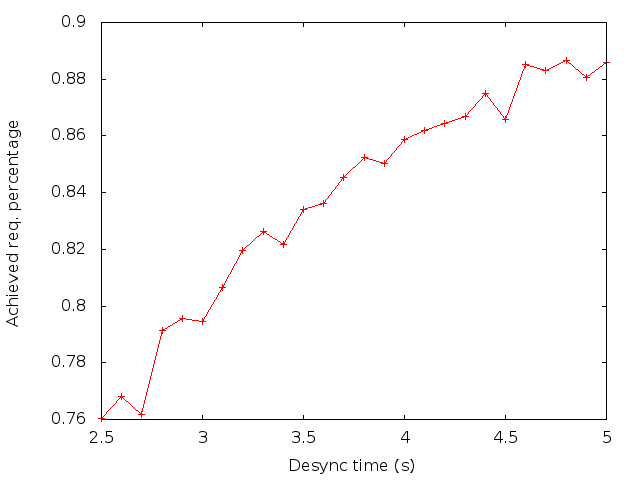
\includegraphics[scale=0.5]{achievedlochexagon6nodescutoff4req3preempt0droponepoint0speed1.png}
    \caption{Percentuale richieste andate a buon fine}
    \label{fig:my_label}
\end{figure}
\begin{figure}[H]
    \centering
    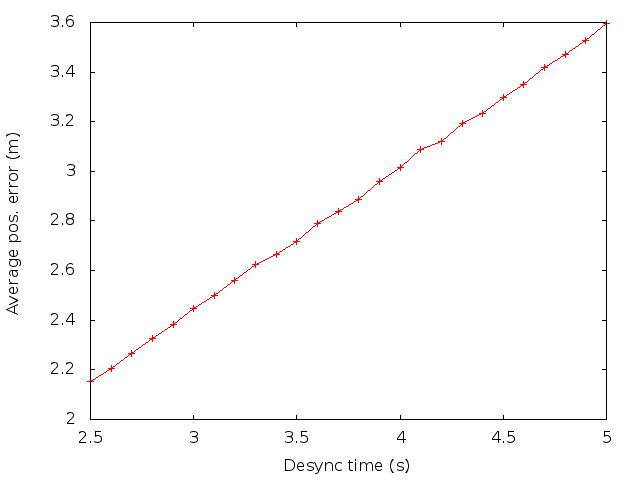
\includegraphics[scale=0.5]{avposerrorhexagon6nodescutoff4req3preempt0droponepoint0speed1.png}
    \caption{Errore medio}
    \label{fig:avposerrorhexagon6nodescutoff4req3preempt0droponepoint0speed1}
\end{figure}
I grafici mappano rispettivamente la percentuale di localizzazioni andate a buon fine e l'errore medio rispetto alla posizione reale, utilizzando come valore sull'asse delle ascisse proprio il massimo tempo di desincronizzazione possibile per i nodi fissi.\newline
\subsubsection{Numero minimo di risposte richieste}
Il funzionamento dell'algoritmo di localizzazione, come verra' esposto in seguito, fa si che' ad un maggior numero di risposte pervenute dai nodi fissi corrisponda un calcolo della posizione del nodo mobile piu' preciso.
Per valutare l'influenza del numero di risposte ricevute sulla precisione della localizzazione e' stato introdotto, come parametro di funzionamento del protocollo, il numero minimo di risposte che vengono richieste per effettuare il calcolo della posizione del nodo mobile.\newline Questo valore non puo' scendere sotto la soglia di 3, numero minimo di risposte necessarie ad effettuare il calcolo. 
Aumentare il valore di questo parametro non aumenta tanto l'accuratezza della posizione calcolata dell'AUV, ma piuttosto aumenta la consistenza del calcolo, facendone diminuire l'errore massimo generato . Tutto questo a scapito  del numero di localizzazioni andate a buon fine (ad esempio , impostando come soglia minima il valore 5, tutti i casi in cui il nodo mobile ricevera' 3 o 4  risposte verranno scartati).\newline
\begin{figure}[H]
    \centering
    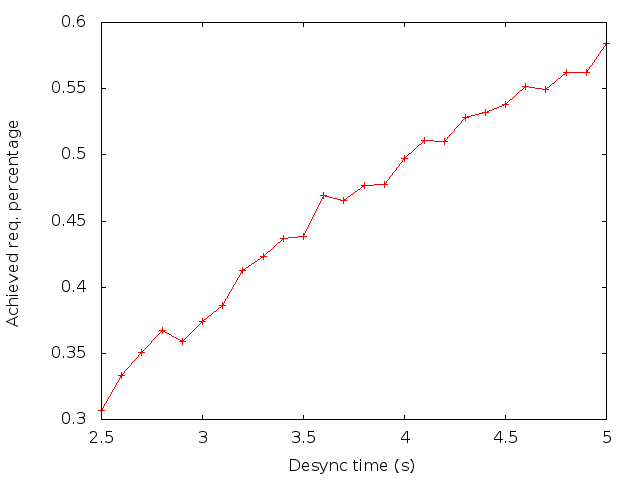
\includegraphics[scale=0.5]{achievedlochexagon6nodescutoff4req5preempt0droponepoint0speed1.png}
    \caption{La percentuale di richieste andate a buon fine diminuisce aumentanto il numero minimo di risposte richiesto (grafico per soglia minima di risposte pari a 5)}
\end{figure}

\begin{figure}[H]
    \centering
    \subfloat[3 risposte]{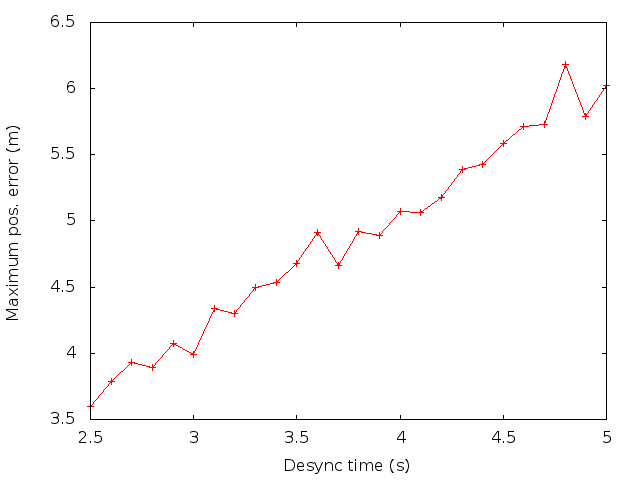
\includegraphics[width=0.4\textwidth]{maxposerrorhexagon6nodescutoff4req3preempt0droponepoint0speed1}\label{fig:f1}}
    \hfill
    \subfloat[5 risposte]{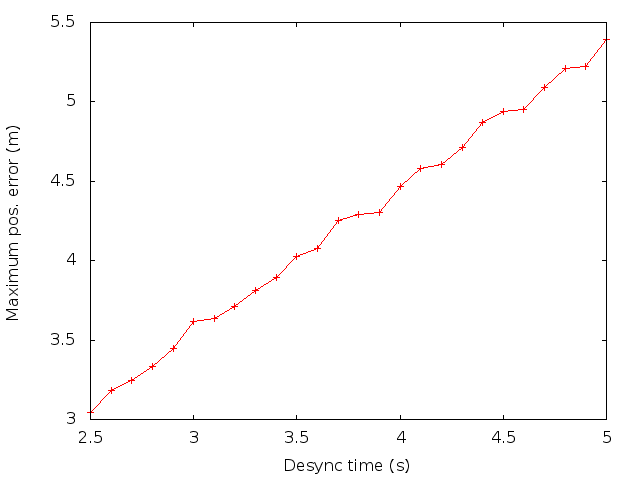
\includegraphics[width=0.4\textwidth]{maxposerrorhexagon6nodescutoff4req5preempt0droponepoint0speed1}\label{fig:f2}}
    \caption{A sinistra, l'andamento dell'errore massimo con numero di richieste minimo impostato a 3. A destra, lo stesso grafico ma con soglia minima impostata a 5. Aspettando due risposte in piu' si guadagnano 0.5 metri sull'errore massimo}
\end{figure}
\subsubsection{Soglia massima numero di condizionamento della matrice del sistema}
\par
Nel calcolo della posizione dell'AUV, ci si trova a dover risolvere un sistema lineare nella forma  \(\textbf{A}\overrightarrow{x} = \overrightarrow{b} \) , ricorrendo a metodologie di approssimazione della soluzione corretta (vedi paragrafo 3.2.4). Per la matrice \(\textbf{A}\) e' possibile definire un valore, detto numero di condizionamento, che ci fornisce una sorta di limite superiore  per l'errore che possiamo ottenere nel calcolo delle coordinate del veicolo mobile. Piu' e' elevato il valore del numero di condizionamento, maggiore e' l'errore che puo' inficiare la validita' della localizzazione. Viene quindi introdotta una soglia massima per il valore del numero di condizionamento, al di sopra della quale la specifica richiesta di localizzazione viene scartata (in modo cosi' da evitare misure influenzate da un errore elevato).
\subsubsection{Modalita' di funzionamento "preemptive"}
Contestualmente all'introduzione del parametro riguardante il numero minimo di risposte richieste, si e' pensato di realizzare una seconda modalita' di funzionamento del protocollo, che verra' indicata col nome di modalita'  ``preemptive''.\newline In questa modalita' viene modificato il  comportamento del nodo mobile rispetto all'attendere lo scadere del timer prima di iniziare il calcolo della propria posizione. Come gia' discusso, cio' comporta un aumento dell'errore nella misurazione della distanza rispetto ai nodi fissi di cui si e' ricevuta risposta, dovuta alla non contemporaneita' del calcolo della posizione rispetto alla ricezione stessa della riposta (in particolare, l'errore sara' tanto maggiore quanto prima si e' ricevuta la risposta rispetto alla fine del timer).\newline
Nella modalita' ``preemptive'' il veicolo, invece di aspettare la fine del timer,  avvia l'algoritmo di localizzazione non appena riceve il numero di risposte indicato dal parametro della soglia minima di risposte necessaria.
Riportiamo il grafico ottenuto sempre con la configurazione a 6 nodi fissi, soglia minima di risposte pari a 3 e velocita' dell'AUV fissata a 1$\frac{m}{s}$. Notiamo come, rispetto al grafico in figura ~\ref{fig:avposerrorhexagon6nodescutoff4req3preempt0droponepoint0speed1}, l'errore medio sia piu' che dimezzato rispetto alla modalita' non "preemptive"
\begin{figure}[H]
    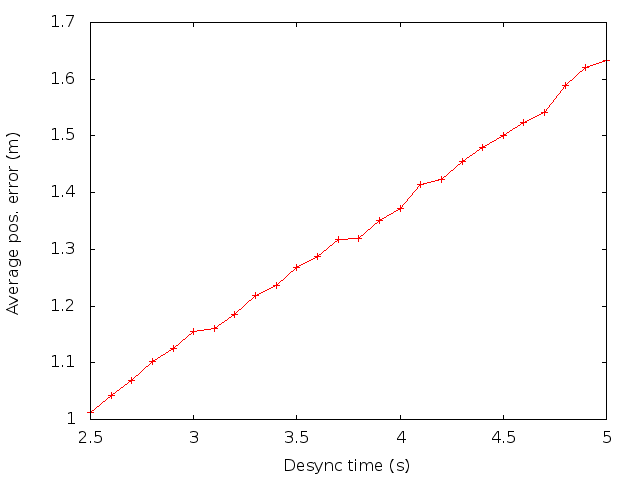
\includegraphics[scale=0.5]{avposerrorhexagon6nodescutoff4req3preempt1droponepoint0speed1.png}
    \centering
\end{figure}

\subsubsection{Modalita' di funzionamento "drop one point"}
\par
Questa modalita' di funzionamento e' strettamente legata alla soglia massima tollerabile introdotta per il valore del numero di condizionamento. Nel corso delle simulazioni, si sono riscontrati valori elevati del numero di condizionamento nei casi in cui il veicolo mobile avesse ricevuto risposte alla propria richiesta di localizzazione da un insieme di nodi nel quale almeno tre dei sensori fissi risultassero quasi allineati sulla stessa retta. Si e' pensato quindi di introdurre una modalita' di funzionamento del protocollo in cui, invece di annullare la localizzazione nel caso del superamento della soglia del numero di condizionamento, l'AUV prova invece ad eliminare dall'insieme delle risposte ricevute quella proveniente da uno dei nodi allineati, in modo da ottenere nel calcolo delle proprie coordinate una matrice con numero di condizionamento al di sotto della soglia di guardia. Per implementare questo comportamento in maniera computazionalmente efficiente, l'AUV scarta iterativamente una delle riposte ottenute (ovviamente solo se ha ricevuto 4 o piu' risposte) e prova ad rieffettuare la localizzazione col sottoinsieme di risposte cosi ottenuto.
\par


\section{Calcolo della posizione}

\subsection{Descrizione generica del calcolo}
La tecnica impiegata per il calcolo della posizione fa uso della metodologia della trilaterazione. La trilaterazione e' un metodo geometrico che permette, utilizzando la geometria delle sfere, il calcolo della posizione assoluta o relativa di un punto in base alla misurazione di alcune specifiche distanze (in questo caso le distanze dai nodi fissi).\newline
Da specificare che, nel caso del nostro nodo mobile, considereremo come nota la profondita' dell'AUV, potendo far uso di un sensore di profondita' di notevole precisione (basato sulla pressione marina).
Quindi, il nostro calcolo verra' effettuato non in tre ma in due dimensioni. 

\subsection{Impostazione matematica del calcolo}
Per ogni risposta che l'AUV riceve da un nodo fisso, possiamo scrivere l'equazione della sfera avente come centro il nodo fisso e come raggio la distanza del veicolo mobile da quel nodo, calcolata tramite il RTT: \newline
\begin{equation}
r_{i} = \sqrt{(x-x_{i})^2+(y-y_{i})^2+(z-z_{i})^2} \qquad (i = 1,...,n)
\end{equation}
\newline
Un metodo banale di risoluzione consisterebbe nel risolvere direttamente il sistema di equazioni quadratiche, operazione computazionalmente onerosa. Inoltre, a causa degli errori introdotti nella misura dei raggi delle sfere, non e' detto che il sistema dato abbia soluzione.
Utilizzeremo invece delle piu' sofisticate tecniche di risoluzione, basate sulla linearizzazione del sistema e su tecniche di approssimazione della soluzione.\newline

\subsection{Linearizzazione del sistema}
In primis, come gia' detto, consideriamo nota la profondita' dell'AUV, $z_{0}$, da cui:
\begin{equation}
(x-x_{i})^2+(y-y_{i})^2 = r'^2_{i}\ ,\ con\ r'^2_{i} = r^2_{i}-(z_{0}-z_{i})^2 \qquad  (i = 1,...,n)
\end{equation}
\newline
Quindi il sistema passa da tre incognite a due sole incognite, il che porta da 4 a 3 il numero minimo delle equazioni necessarie alla risoluzione del sistema.
Utilizziamo indifferentemente una delle equazioni per linearizzare il sistema, in questo caso la prima equazione, da cui avremo:\newline
\begin{equation}
(x-x_{1}+x_{1}-x_{i})^2+(y-y_{1}+y_{1}-y_{i})^2 =  r'^2_{i} \qquad  (i = 2,...,n)
\end{equation}
\newline
Da cio' otterremo il seguente sistema:\newline
\begin{equation}
2(x_{1}-x_{i})+2(y_{1}-y_{i}) =  r'^2_{i}-r'^2_{1}-x^2_{i}-y^2_{i}+x^2_{1}+y^2_{1} \qquad (i = 2,...,n)
\end{equation}

A partire da un sistema di $n$ equazioni di secondo grado in 3 incognite, abbiamo ottenuto un sistema lineare in 2 incognite con $n$-1 equazioni.\newline Ora diviene chiaro il perche' della soglia minima di risposte necessarie fissata a 3, che permette in finale di ottenere un sistema lineare di 2 equazioni in 2 incognite.\newline Il sistema, nella forma $\textbf{A}\overrightarrow{x}=\overrightarrow{b}$, potrebbe essere risolto direttamente risolvendo 2 delle equazioni in esso presenti. Cio' non e' detto sia possibile ne' ci viene garantito che si ottenga in tal modo il risultato piu' preciso. Adotteremo quindi una diversa approssimata di risoluzione, nota come metodo dei minimi quadrati.\newline

\subsection{Metodo dei minimi quadrati}
Il metodo dei minimi quadrati e' un metodo di ottimizzazione il cui scopo e' individuare, dato un insieme di dati (in questo caso punti del piano), una funzione che ben approssimi quei valori. Nel dettaglio, si tratta di trovare la funzione che minimizza la somma dei quadrati della differenza fra i dati osservati e i valori della  stessa funzione approssimante (da cui il nome del metodo).\newline
In questo caso, il valore da minimizzare e': \newline
\begin{equation}
S = \overrightarrow{r}^T\overrightarrow{r} = (\overrightarrow{b}-\textbf{A}\overrightarrow{x})^T(\overrightarrow{b}-\textbf{A}\overrightarrow{x})
\end{equation}
\newline
Da questa formula si arriva all'equazione normale:\newline
\begin{equation}
\textbf{A}^T\textbf{A}\overrightarrow{x} = \textbf{A}^T\overrightarrow{b}
\end{equation}
\newline
A questo punto, se la matrice $\textbf{A}$ non e' singolare, si puo' risolvere direttamente l'equazione:\newline
\[\overrightarrow{x} = (\textbf{A}^T\textbf{A})^{-1}\textbf{A}^T\overrightarrow{b}\]
La risoluzione diretta dell'equazione normale non garantisce risultati precisi. La causa di quest'imprecisione e' da ritrovarsi nel numero di condizionamento della matrice. Il sistema lineare $\textbf{A}\overrightarrow{x} = \overrightarrow{b}$ puo' essere in realta' riscritto, per via degli errori nella misurazione delle distanze, come: \newline
\begin{equation}
\textbf{A}\overrightarrow{x} = \overrightarrow{b} \rightarrow \textbf{A}(\overrightarrow{x}+\delta\overrightarrow{x}) = (\overrightarrow{b}+\delta\overrightarrow{b})
\end{equation}
\newline
in cui $\delta\overrightarrow{b}$ e' proprio l'errore introdotto dall'imprecisione nelle misurazioni.
In tal modo possiamo scrivere l'errore nel calcolo in forma matriciale:\newline
\begin{equation}
\textbf{A}\delta\overrightarrow{x} = \delta\overrightarrow{b}
\end{equation}
\newline
da cui, passando alla norma: \newline
\begin{equation}
||\delta\overrightarrow{x}|| \leq ||\textbf{A}^{-1}|| \cdot ||\delta\overrightarrow{b}||
\end{equation}
Definiamo a questo punto il numero di condizionamento come la quantita': \newline
\begin{equation}
\kappa (\textbf{A}) = ||\textbf{A}|| ||\textbf{A}^{-1}|| 
\end{equation}
\newline
Finalmente giungiamo all'equazione: \newline
\begin{equation}
\frac{||\delta\overrightarrow{x}||}{||\overrightarrow{x}||} \leq  \kappa (\textbf{A}) \frac{||\delta\overrightarrow{b}||}{||\overrightarrow{b}||}
\end{equation}
Questa e' la stima dell'errore relativo.Esso dipende fortemente dagli errori presenti nelle misurazioni delle distanze, che possono essere amplificati al massimo secondo un fattore che dipende dalla natura stessa della matrice, appunto il numero di condizionamento. Indipendentemente dall'errore presente nel calcolo delle distanze dai nodi fissi, un basso numero di condizionamento ci garantisce che l'errore nelle misurazioni non si propaghera' in maniera esagerata mentre, al contrario, un alto valore di questo parametro potrebbe rendere inutilizzabile la posizione calcolata anche in presenza di un piccolo errore sui termini noti del sistema.\newline
Viene appunto introdotto, quindi, un parametro di funzionamento del protocollo che rappresenta la soglia massima accettabile per il valore del numero di condizionamento della matrice \textbf{A}, scartando i risultati in caso di superamento di tale soglia.

\section{Considerazioni sull'utilizzo e testing del protocollo}
\par
Nella sezione successiva dell'elaborato verranno presentati i dati relativi ai test di simulazione del protocollo, dei quali vogliamo sottolineare quali siano stati gli obbiettivi che hanno guidato tutta la fase di testing.
\par
I parametri d'interesse nella valutazione  dell'algoritmo sono stati essezialmente tre:
\begin{itemize}
\item La percentuale di localizzazioni andate a buon fine rispetto al numero di localizzazioni tentate
\item L'errore medio ottenuto nel calcolo della posizione dell'AUV
\item L'errore massimo riscontrato nel valore della posizione calcolata
\end{itemize}
Ovviamente, obbiettivo principale delle simulazioni e' stato valutare in quali configurazioni di funzionamento del protocollo si riuscisse a massimizzare la percentuale di richieste di localizzazione effettuate con successo posto che, ancor prima di considerazioni sull'errore di posizionamento, fosse importante ottenere una buona percentuale d'affidabilita' del protocollo stesso.  In secondo luogo, e' stato ovviamente rilevante valutare quale fosse l'errore medio ottenuto sulla localizzazione, considerando l'importanza di questo valore come misura della bonta' del protocollo e di un suo eventuale utilizzo in un contesto applicativo reale. Il terzo fattore indicato (l'errore massimo) puo' essere considerato come un indicatore della varianza dell'errore insito nella localizzazione. In uno scenario di concreto utilizzo del protocollo, la misurazione della posizione di un veicolo mobile puo' essere ulteriormente raffinata facendo ricorso a filtri matematici (es. filtro di Kalman) e tecniche di dead-reckoning (stima della posizione  di un veicolo in base ad una posizione precedente nel tempo e ad informazioni sul movimento del veicolo stesso) in grado di correggere eventuali valori troppo elevati ottenuti per l'errore massimo.



\chapter{Simulazioni}
In questo capitolo vengono descritte le simulazioni effettuate per testare il funzionamento del protocollo di localizzazione in diversi scenari. \newline Le simulazioni sono state effettuate immaginando una rete costituita da un AUV, fisso in un punto o in movimento, e da un certo numero di nodi fissi, variabili nel numero di 4, 6 o 8 nodi.

\section{Ambiente simulativo}

\subsection{Parametri generali della simulazione}
\par
Le simulazioni vengono effettuate considerando le trasmissioni acustiche modulate secondo modulazione BPSK (PSK Bifase). La potenza delle trasmissione e' di 180 dB rispetto al valore base di 1 $\mu$Pa a distanza di 1 $m$. La frequenza centrale per la trasmissione del segnale e' di 25 kHz, con un'ampiezza di banda impiegata di 4 kHz. Il bitrate che si ottiene con questi valori e' di 860 $\frac{bit}{s}$, confrontabile con quello di modem acustici commercialmente disponibili (EvoLogics, Teledyne, Sonardyne).
Nelle simulazioni effettuate, la velocita' di spostamento verticale dell'AUV e' stata impostata a 0.86 \(\frac{m}{s}\), mentre il valore della velocita' angolare utilizzato e' di 1.23 \(\frac{rad}{s}\) ( i valori riportati dai progettisti di MARTA).\newline La velocita' di spostamento in linea retta e' stato uno dei parametri la cui variazione ed il conseguente effetto sull'efficacia del protocollo sono stati considerati di primario interesse. Abbiamo considerato le situazioni in cui l'AUV fosse fermo in mezzo alla rete dei nodi fissi (quindi velocita' di 0 \(\frac{m}{s}\)) e quelle in cui l'AUV si spostasse rispettivamente ad 1 e 2 \(\frac{m}{s}\)). La velocita' di 1 $\frac{m}{s}$ e' riferibile alla velocita' reale con cui un AUV si sposterebbe in una missione sul campo, mentre con il valore di 2 $\frac{m}{s}$ si e' voluta simulare la situazione di velocita' di punta dichiarata di MARTA (4 nodi, circa 2.05 $\frac{m}{s}$). In tutte e tre i possibili scenari di movimento, l'AUV effettua una richiesta di localizzazione ogni 20 secondi, generando un pacchetto con payload vuoto.
\par
Ciascuna configurazione di una simulazione e' caratterizzabile da una quintupla di parametri:
\begin{itemize}
    \item Velocita' dell'AUV
    \item Soglia per numero di condizionamento
    \item Abilitazione modalita' "preemptive"
    \item Abilitazione modalita' "drop one point"
    \item Topologia dei nodi fissi utilizzata
\end{itemize}
Abbiamo gia' discusso i valori utilizzati per la velocita'. Il valore della soglia del numero di condizionamento e' stato fatto variare in un range di valori interi che va da 4 a 10. Per ciascuna di queste configurazioni, e' stata fatta una simulazione variando il valore massimo del timer di desincronizzazione dei nodi fissi da 2.5 $s$ a 5 $s$, con un passo di 0.1 $s$

\subsection{Topologie dei nodi fissi}
Sono state utilizzate tre diverse topologie di rete. Tutte e tre le topologie hanno un diametro (distanza massima fra due nodi fissi) di 200 metri, valore che e' stato utilizzato per il calcolo del delay di propagazione considerato nel timer di invio dell'AUV. Come suggerito da varie implementazioni di sistemi di localizzazione LBL, i sensori fissi sono stati posizionati ai contorni dell'area delle operazioni dell'AUV. \newline
\subsubsection{Topologia 4 nodi}
Nella topologia a 4 nodi, i nodi fissi sono disposti ai vertici di un parallelogramma, a diverse altezze, in modo che il piano di giacenza della figura risulti inclinato rispetto al piano orizzontale. Visti dall'alto, i nodi costituiscono i vertici di un quadrato.
\begin{figure}[H]
    \centering
    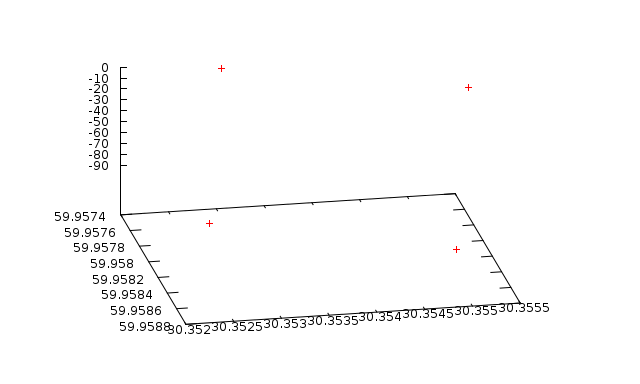
\includegraphics[width=\linewidth]{squaretopology.png}
    \caption{Topologia a 4 nodi}
    \label{fig:my_label}
\end{figure}
Questa e' la topologia di maggior interesse visto che, dato il costo del dispiegamento di sensori fissi dotati di modem acustico, si tende a ridurre al minimo il numero stesso di questi nodi.

\subsubsection{Topologia 6 nodi}
Nella topologia a 6 nodi, i nodi fissi sono disposti ai vertici di quello che, visto dall'alto, risulta essere un esagono. Tutti i nodi sono ad altezze diverse fra loro.   
\begin{figure}[H]
    \centering
    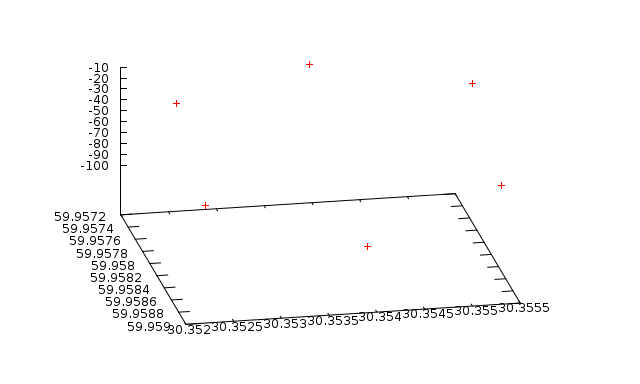
\includegraphics[width=\linewidth]{topologyhexagon.png}
    \caption{Topologia a 6 nodi}
    \label{fig:my_label}
\end{figure}
\subsubsection{Topologia 8 nodi}
Nella topologia a 8 nodi, i nodi fissi sono disposti ai vertici di un ottagono, a diverse altezze.
\begin{figure}[H]
    \centering
    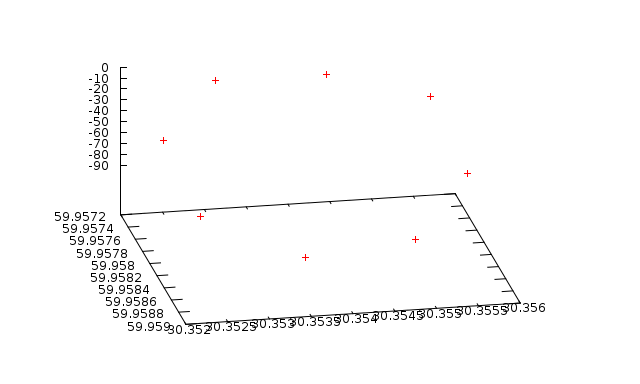
\includegraphics[width=\linewidth]{topologyoctagon.png}
    \caption{Topologia a 8 nodi}
    \label{fig:my_label}
\end{figure}

\section{Risultati della simulazione}
In questa sezione vengono riportati i risultati delle simulazioni svolte per le diverse topologie di rete sopra discusse. In ciascun grafico verranno riportati gli andamenti delle misurazioni impostando la soglia del valore di condizionamento rispettivamente ai valori 4, 7 e 10 (gli estremi del range simulativo ed il valore mediano).  
\subsection{Topologia a 4 nodi}
In primis, riportiamo i grafici per quanto concerne la situazione di AUV fermo nel punto "centrale" della topologia (proiettando i punti su piano x-y). Questa configurazione serve a simulare la modalita' operativa in cui, prima di effettuare la localizzazione, si obbliga il veicolo mobile a fermarsi. Se cio' puo' comportare una perdita di tempo rispetto alla missione cui e' assegnato l'AUV, di contro sia l'accuratezza che la precisione della localizzazione ottenuta sono elevate.

\begin{figure}[H]
    \centering
    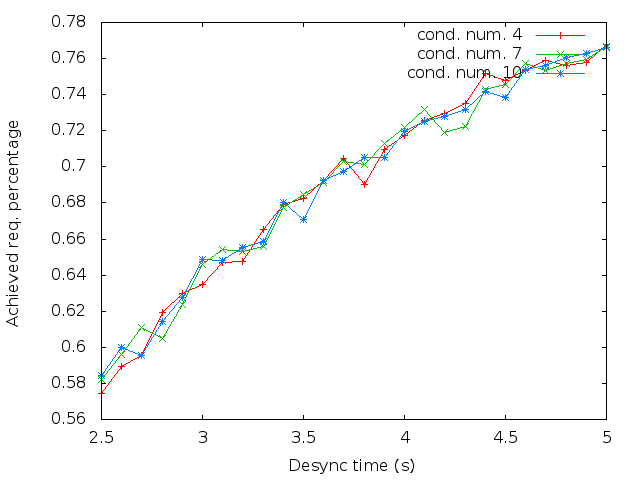
\includegraphics[scale=0.5]{squaresimulation/achievedlocpreempt0drop0speed0.png}
    \caption{Localizzazioni andate a buon fine}
    \label{fig:squaresimulation/achievedlocpreempt0drop0speed0}
\end{figure}

Il grafico ci anticipa, come si osservera' nel resto della sezione dedicata a questa topologia, l'irrilevanza della soglia del numero di condizionamento. Difatti trovandosi le proiezioni sul piano orizzontale delle posizioni dei nodi fissi ai vertici di un quadrato, l'allineamento fra queste posizioni e' minimo e di conseguenza anche il valore del numero di condizionamento sara' basso. Aumentando il valore del timer di desincronizzazione delle risposte, aumenta la percentuale di localizzazioni andate a buon fine, come ci si aspetta. E' da considerare, com'anche nelle successive simulazioni, che l'AUV si trova fermo in posizione quasi equidistante dai nodi fissi, da cui la necessita' di aumentare di molto il valore del tempo di desincronizzazione per evitare collisioni. Le stesse richieste effettuate in una posizione piu' decentrata avrebbero sicuramente necessitato di un minor valore del timer per ottenere pari risultati in termini di successo della localizzazione.
Per quanto riguarda l'errore medio e l'errore massimo sulla posizione calcolata, esso e' praticamente nullo, essendo entrambi minori di 10 $cm$.
In questa particolare situazione, variare modalita' di funzionamento del protocollo o soglia minima di richieste necessarie non causa praticamente mutazioni nei risultati ottenuti.

\begin{figure}[H]
    \centering
    \subfloat[Errore medio]{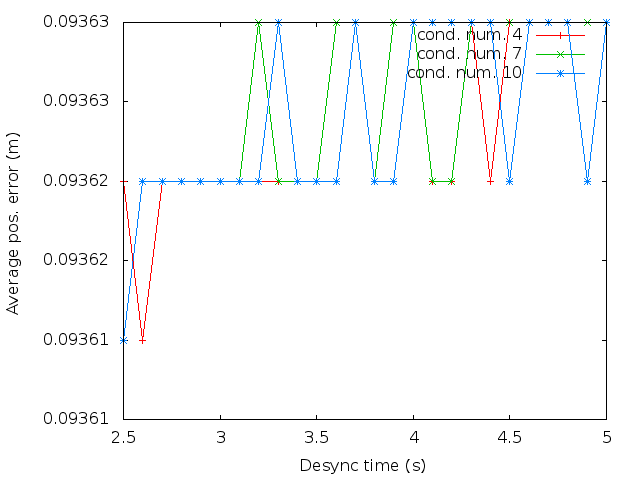
\includegraphics[width=0.4\textwidth]{squaresimulation/avposerrorpreempt0drop0speed0.png}
    \label{fig:squaresimulation/avposerrorpreempt0drop0speed0.png}}
    \hfill
    \subfloat[Errore massimo]{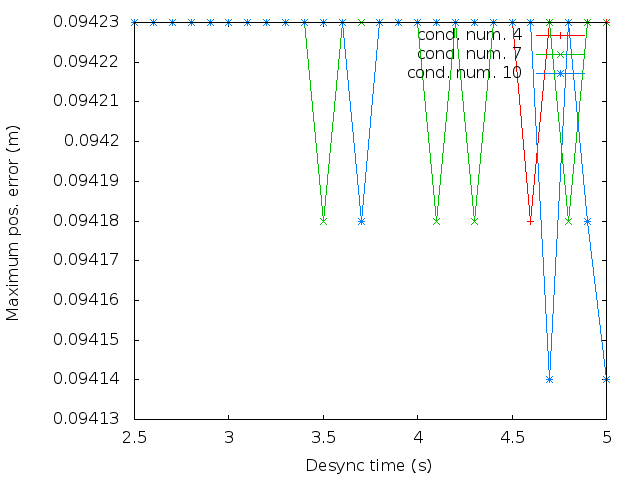
\includegraphics[width=0.4\textwidth]{squaresimulation/maxposerrorpreempt0drop0speed0.png}
    \label{fig:squaresimulation/maxposerrorpreempt0drop0speed0}}
\end{figure}

Di maggiore interesse sono i risultati ottenuti facendo muovere l'AUV a velocita' di 1 $\frac{m}{s}$. Riportiamo subito i grafici, confrontando la configurazione in cui si richiedono tre riposte con quella in cui ne richiediamo quattro.

\begin{figure}[H]
    \centering
    \subfloat[3 richieste]{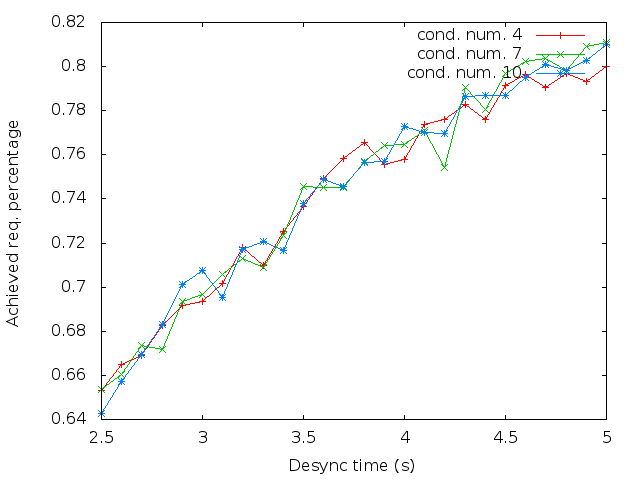
\includegraphics[width=0.4\textwidth]{squaresimulation/achievedlocreq3preempt0drop0speed1.png}
    \label{fig:squaresimulation/achievedlocreq3preempt0drop0speed1}}
    \hfill
    \subfloat[4 richieste]{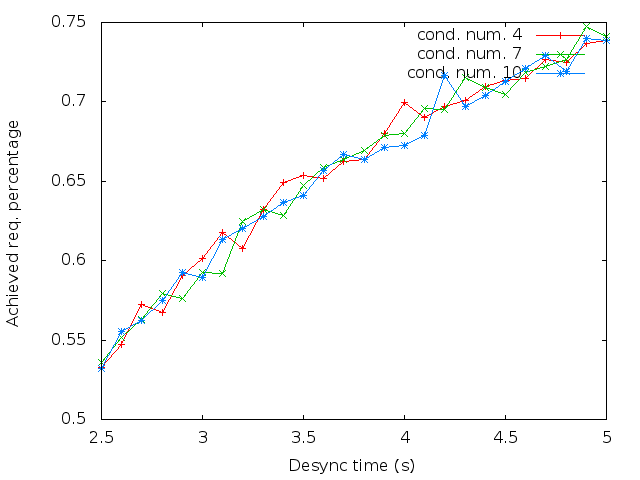
\includegraphics[width=0.4\textwidth]{squaresimulation/achievedlocreq4preempt0drop0speed1.png}
    \label{fig:squaresimulation/achievedlocreq3preempt0drop0speed1}}
    \caption{Percentuale di richieste portate a termine}
\end{figure}

\begin{figure}[H]
    \centering
    \subfloat[3 richieste]{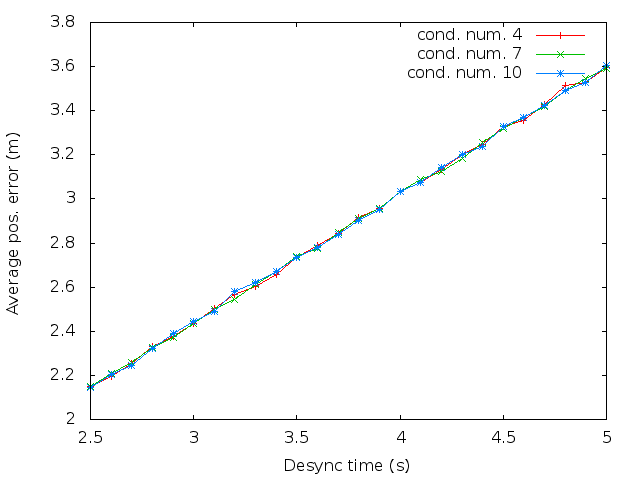
\includegraphics[width=0.4\textwidth]{squaresimulation/avposerrorreq3preempt0drop0speed1.png}
    \label{fig:squaresimulation/avposerrorreq3preempt0drop0speed1}}
    \hfill
    \subfloat[4 richieste]{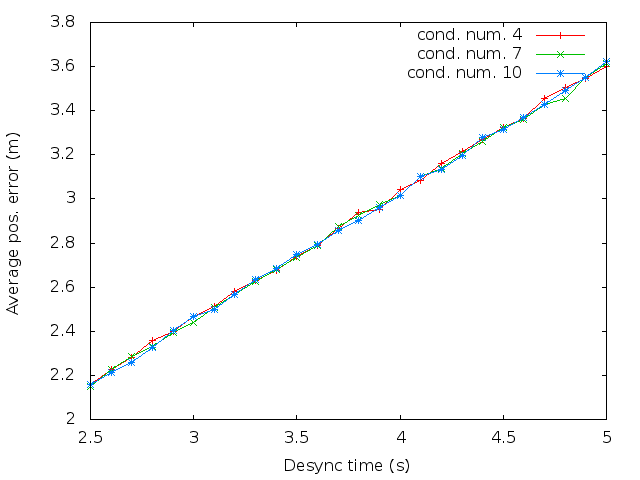
\includegraphics[width=0.4\textwidth]{squaresimulation/avposerrorreq4preempt0drop0speed1.png}
    \label{fig:squaresimulation/avposerrorreq4preempt0drop0speed1}}
    \caption{Errore medio}
\end{figure}

\begin{figure}[H]
    \centering
    \subfloat[3 richieste]{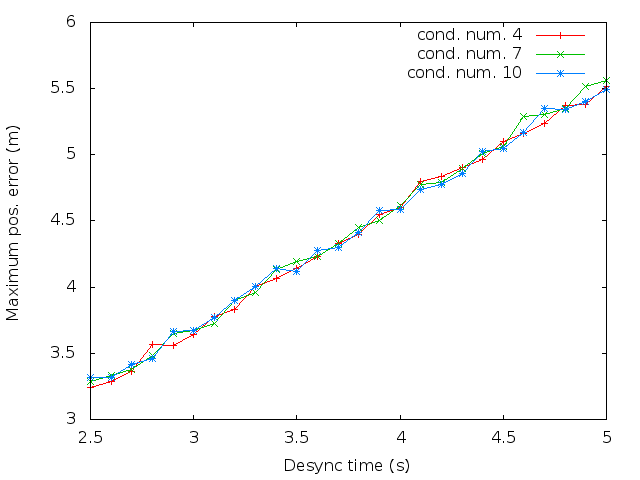
\includegraphics[width=0.4\textwidth]{squaresimulation/maxposerrorreq3preempt0drop0speed1.png}
    \label{fig:squaresimulation/maxposerrorreq3preempt0drop0speed1}}
    \hfill
    \subfloat[4 richieste]{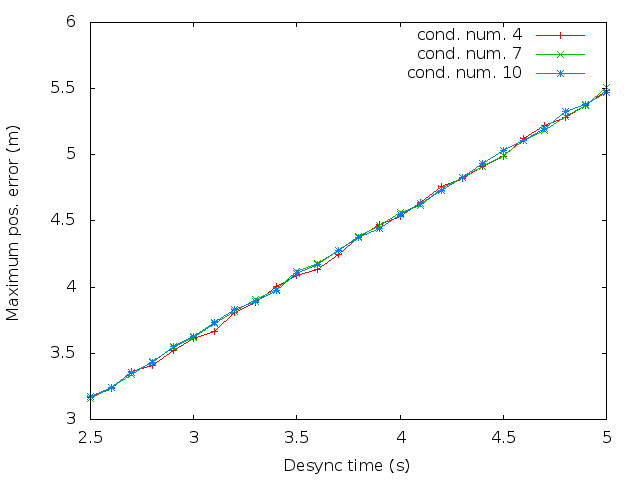
\includegraphics[width=0.4\textwidth]{squaresimulation/maxposerrorreq4preempt0drop0speed1.png}
    \label{fig:squaresimulation/maxposerrorreq4preempt0drop0speed1}}
    \caption{Errore massimo}
\end{figure}

In primis, si evince come l'attesa di una risposta in piu' rispetto al numero minimo di 3 non sortisca effetti positivi degni di nota. Al contrario, causa la diminuzione della percentuale di localizzazioni riuscite (di circa il 5 per tempo di desincronizzazione pari a 4.5 $s$\%).
Ci limitiamo quindi all'analisi della simulazione fatta attendendo 3 risposte.
Potendo considerare come sufficiente una percentuale di localizzazioni riuscite pari al 70\%, questo risultato viene raggiunto con un tempo di desincronizzazione di poco piu' di 3 secondi. Per questo valore, l'errore medio risulta essere di circa 2.5 $m$ mentre l'errore massimo e' di circa 3.7 $m$.
Col valore massimo considerato per il timer (5 $s$), questi due valori salgono a 3.6 e 5.5 $m$ rispettivamente, con un guadagno sulle localizzazioni positivamente effettutate di circa un 10\%.

E' stato interessante a questo punto verificare se la modalita' "preemptive" potesse in qualche modo migliorare i risultati fin qui ottenuti.
Se l'andamento della percentuale delle localizzazioni riuscite non viene modificato, si ottiene altresi' un notevole miglioramento delle prestazioni per quanto riguarda l'errore nel calcolo delle coordinate dell'AUV.

\begin{figure}
    \centering
    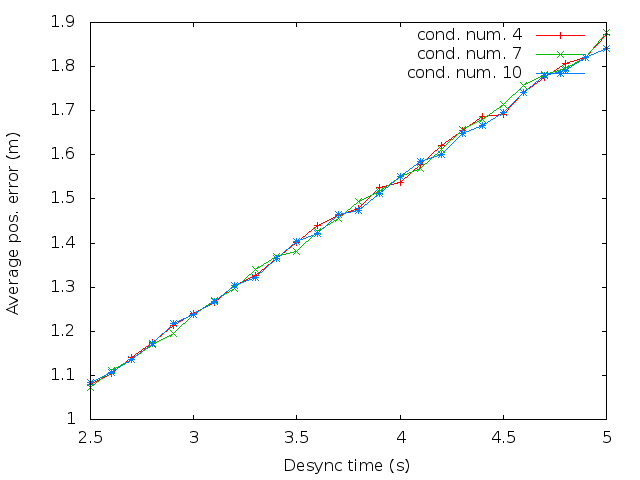
\includegraphics[scale=0.5]{squaresimulation/avposerrorreq3preempt1drop0speed1.png}
    \caption{Errore medio}
    \label{fig:squaresimulation/avposerrorreq3preempt1drop0speed1}
\end{figure}

\begin{figure}
    \centering
    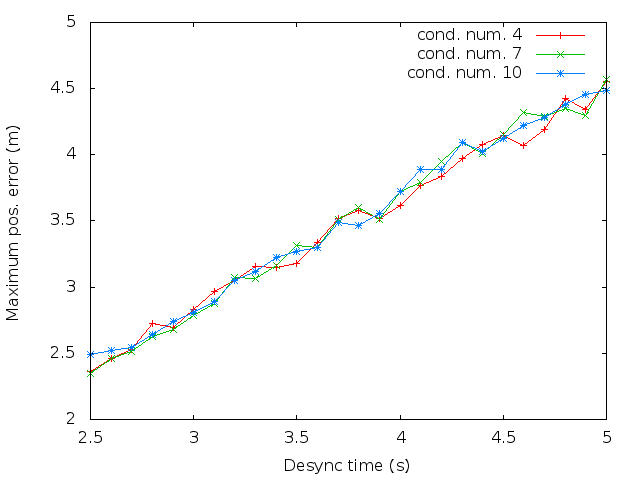
\includegraphics[scale=0.5]{squaresimulation/maxposerrorreq3preempt1drop0speed1.png}
    \caption{Errore massimo}
    \label{fig:squaresimulation/maxposerrorreq3preempt1drop0speed1}
\end{figure}

Il miglioramento rispetto alla modalita' normale e' evidente. Considerando di nuovo la soglia del 70\% di localizzazioni riuscite, in corrispondenza di quel valore abbiamo un errore medio sulle coordinate calcolate del veicolo di circa 1.25 $m$ ed un errore massimo di circa 2.8 $m$. Prendendo il massimo valore del timer di desincronizzazione, l'errore medio comunque non sale oltre i 2 $m$, meno della meta' del valore in ~\ref{fig:squaresimulation/maxposerrorreq3preempt0drop0speed1}.
Come ci si aspettava, il movimento dell'AUV durante l'attesa dello scadere del timer per effettuare il calcolo della posizione e' uno dei fattori che piu' influenzano negativamente la precisione della localizzazione. La modalita' "preemptive", che ne diminuisce l'effetto, genera quindi un netto miglioramento nelle prestazioni del protocollo.
Riportiamo ora i risultati considerando un AUV che si stia movendo al doppio della velocita' or ora considerata, ovverro 2 $\frac{m}{s}$.
Di nuovo, la configurazione in cui si richiedono un minimo di 4 risposte non genera' risultati diversi dalla versione a 3 risposte.
Confrontiamo i risultati in modalita' preemptive e non preemptive, per evidenziare ulteriormente la bonta' di tale modalita'.

\begin{figure}[H]
    \centering
    \subfloat[Non Preemptive]{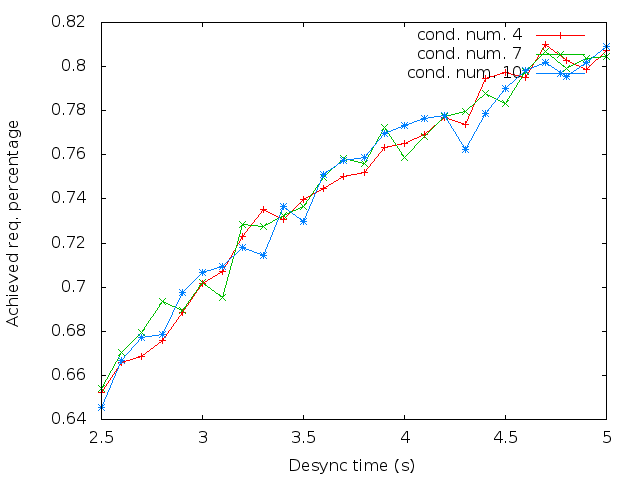
\includegraphics[width=0.4\textwidth]{squaresimulation/achievedlocreq3preempt0drop0speed2.png}
    \label{fig:squaresimulation/achievedlocreq3preempt0drop0speed2}}
    \hfill
    \subfloat[Preemptive]{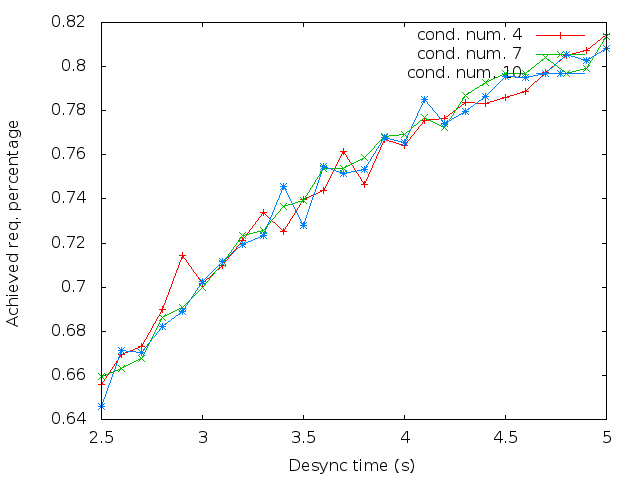
\includegraphics[width=0.4\textwidth]{squaresimulation/achievedlocreq3preempt1drop0speed2.png}
    \label{fig:squaresimulation/achievedlocreq3preempt1drop0speed2}}
    \caption{Localizzazioni riuscite}
\end{figure}

\begin{figure}[H]
    \centering
    \subfloat[Non Preemptive]{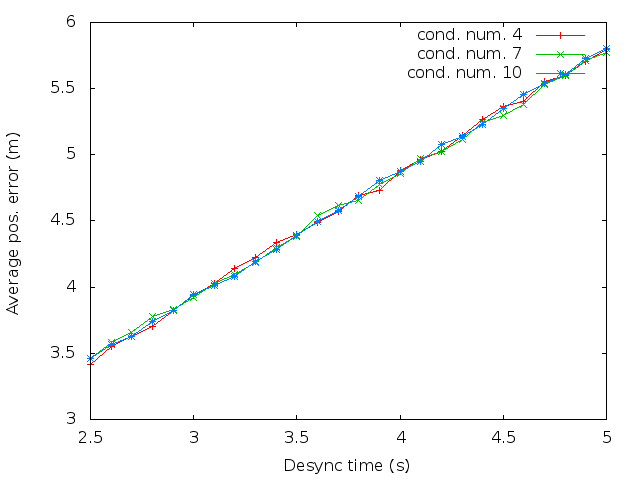
\includegraphics[width=0.4\textwidth]{squaresimulation/avposerrorreq3preempt0drop0speed2.png}
    \label{fig:squaresimulation/avposerrorreq3preempt0drop0speed2}}
    \hfill
    \subfloat[Preemptive]{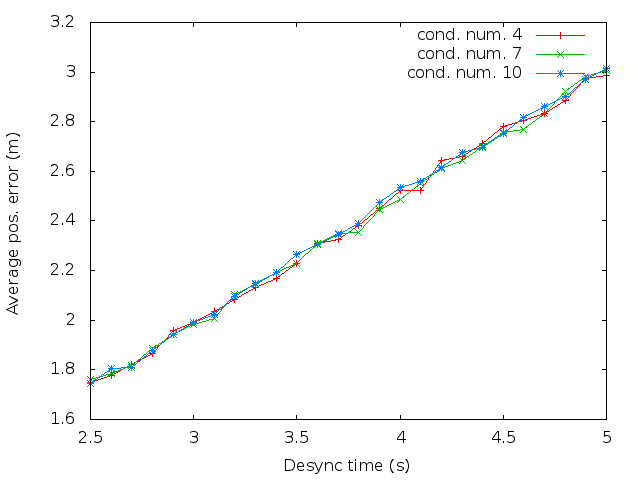
\includegraphics[width=0.4\textwidth]{squaresimulation/avposerrorreq3preempt1drop0speed2.png}
    \label{fig:squaresimulation/avposerrorreq3preempt1drop0speed2}}
    \caption{Errore medio}
\end{figure}

\begin{figure}[H]
    \centering
    \subfloat[Non Preemptive]{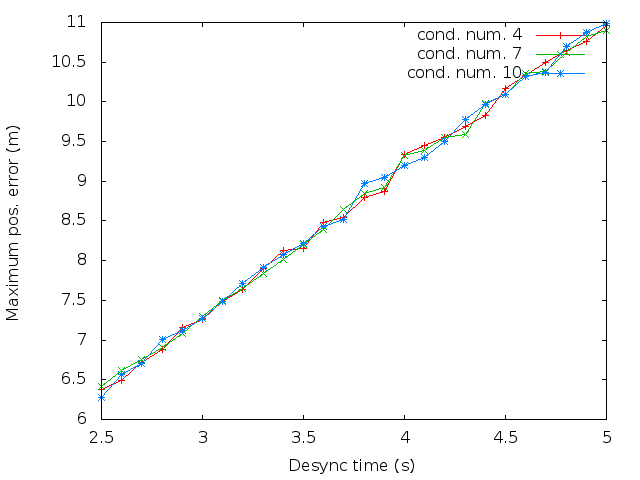
\includegraphics[width=0.4\textwidth]{squaresimulation/maxposerrorreq3preempt0drop0speed2.png}
    \label{fig:squaresimulation/maxposerrorreq3preempt0drop0speed2}}
    \hfill
    \subfloat[Preemptive]{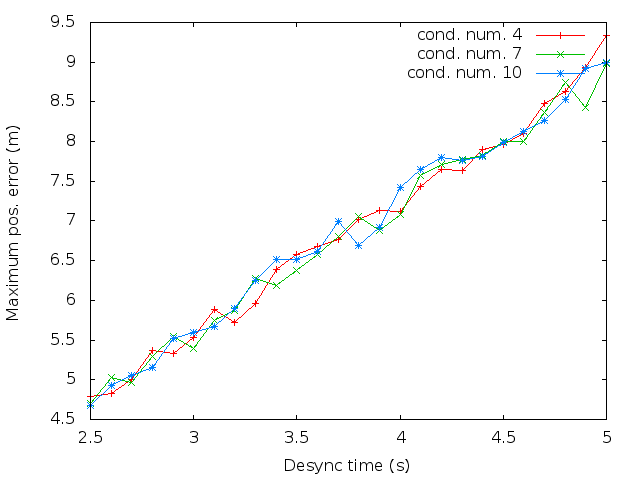
\includegraphics[width=0.4\textwidth]{squaresimulation/maxposerrorreq3preempt1drop0speed2.png}
    \label{fig:squaresimulation/maxposerrorreq3preempt1drop0speed2}}
    \caption{Errore massimo}
\end{figure}
Anche alla velocita' di punta di 2 $\frac{m}{s}$, si potrebbe garantire, con probabilita' di riuscita della localizzazione del 70\%, un errore sulla posizione di circa 2 $m$ ed errore massimo di 5.5 $m$, valori non da sottovalutare dato che si tratta di una velocita' abbastanza elevata per questo tipo di dispositivi. 

\subsection{Topologia a 6 nodi}
Passiamo ora in rassegna i risultati ottenuti con la topologia a 6 nodi fissi.
Nelle simulazioni ci si aspettava che l'aggiunta di due nodi fissi avrebbe migliorato, se non l'errore della posizione calcolata rispetto alla posizione reale, almeno la percentuale di localizzazioni andata a buon fine, essendoci due nodi in piu' da cui l'AUV potesse ricevere risposta. Effettivamente, imponendo la soglia minima di risposte pari a 3 e AUV fermo, rispetto alla configurazione a 4 nodi fissi c'e' un netto aumento della percentuale delle richieste di localizzazione riuscite:
\begin{figure}[H]
    \centering
    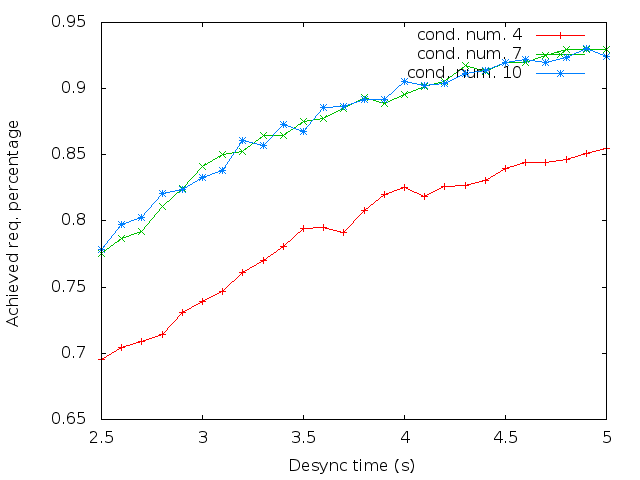
\includegraphics[scale=0.5]{hexagonsimulation/achievedlocreq3preempt0drop0speed0.png}
    \caption{Percentuale localizzazioni riuscite}
    \label{fig:hexagonsimulation/achievedlocreq3preempt0drop0speed0}
\end{figure}
La media dell'errore sulla posizione calcolata, come in ~\ref{fig:squaresimulation/avposerrorpreempt0drop0speed0.png}, e' all'incirca di 10 $cm$, mentre l'errore massimo misurato e' di circa 20 $cm$ con numero di condizionamento massimo uguale a 4 mentre risulta essere di circa 30 $cm$ negli altri due casi.
Rispetto alla topologia a 4 nodi, notiamo come in questa situazione il valore utilizzato come soglia per il numero di condizionamento influenzi in maniera decisiva il funzionamento del protocollo. Difatti, nella topologia a 6 nodi fissi, e' probabile che in alcuni casi l'AUV riceva risposte da nodi fra loro vicini ed allineati (l'angolo fra 3 nodi consecutivi di un esagono e' di 120 gradi, mentre per il quandrato sono 90 gradi). Di qui l'aumento del valore medio del numero di condizionamento, che in certi casi si trova la soglia impostata. A questo fenomeno abbiamo ricondotto la differenza fra il grafico con soglia pari a 4 e quello con soglia pari a 7 e 10, dove invece le richieste non andate a buon fine sono quasi tutte da imputare a collisioni fra le risposte inviate dai nodi fissi.
Si e' cercata quindi una soluzione che garantisse la maggior precisione di una soglia bassa per il numero di condizionamento combinando al tempo stesso la percentuale di localizzazioni riuscite.
Da qui nasce la modalita' "droponepoint", che da' all'AUV la possibilita' di scartare iterativamente una delle risposte ricevute e ripetere il calcolo della propria posizione, sperando di rientrare all'interno della soglia prestabilita per il numero di condizionamento. Riportiamo il grafico del funzionamento del protocollo nella situazione analoga a quella presentata nel grafico precedente, ma con la modalita' "droponepoint" attivata:
\begin{figure}[H]
    \centering
    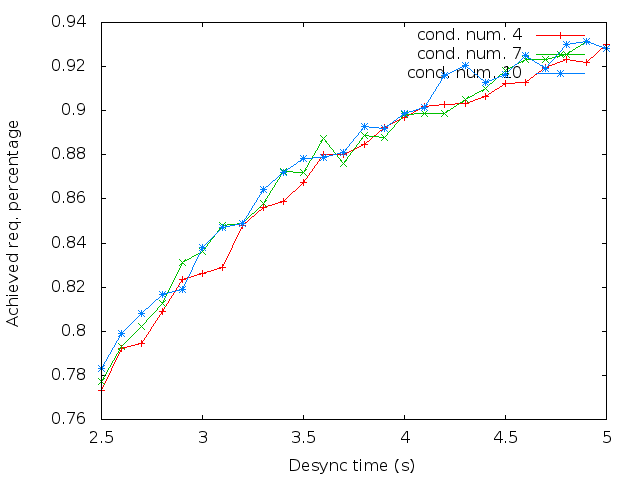
\includegraphics[scale=0.5]{hexagonsimulation/achievedlocreq3preempt0drop1speed0.png}
    \caption{Percentuale localizzazioni riuscite}
    \label{fig:hexagonsimulation/achievedlocreq3preempt0drop1speed0}
\end{figure}
Con la modalita' attivata, la percentuale di localizzazioni riuscite per valore soglia pari a 4 raggiunge quella degli altri due grafici, mantenendo inalterati i valori dell'errore medio e dell'errore massimo. 
Come per la topologia a 4 nodi, aumentare la soglia minima di richieste con il veicolo fermo non migliora l'efficienza del protocollo. Al contrario, la percentuale di localizzazioni andate a buon fine diminuisce di molto, mentre l'errore medio e' piu' o meno uguale. Migliora solamente l'errore massimo (diviene anch'esso di poco superiore ai 10 $cm$), in conformita' col comportamento previsto dal metodo matematico utilizzato per calcolare le coordinate dell'AUV (un maggior numero di risposte implica un numero di condizionamento minore e dunque una minor propagazione dell'errore sulle distanza nel calcolo della posizione).
Consideriamo ora le situazioni in cui imposto la soglia minima di risposte rispettivamente a 3 e 4, facendo muovere l'AUV ad 1 $\frac{m}{s}$.
Riportiamo direttamente i grafici ottenuti attivando la modalita' "preemptive". Confrontiamo i risultati ottenuti utilizzando solamente questa modalita' e quelli ottenuti in combinazione con la modalita' "droponepoint", attivata per la configurazione con soglia minima di risposte impostata a 4.


\begin{figure}[H]
    \centering
    \subfloat[Non Droponepoint]{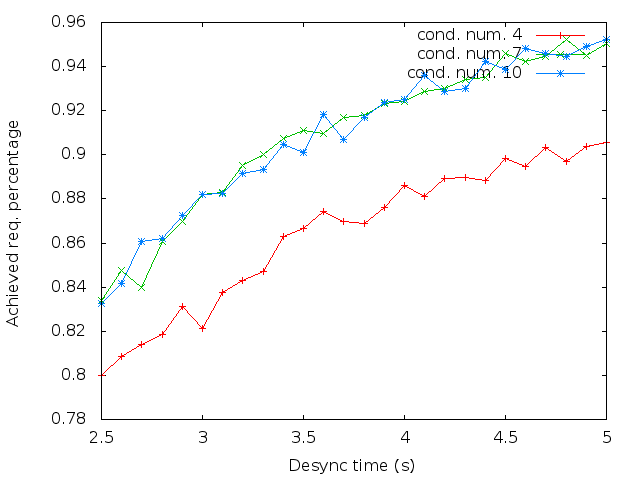
\includegraphics[width=0.4\textwidth]{hexagonsimulation/achievedlocreq3preempt1drop0speed1.png}
    \label{fig:hexagonsimulation/achievedlocreq3preempt1drop0speed1}}
    \hfill
    \subfloat[Droponepoint]{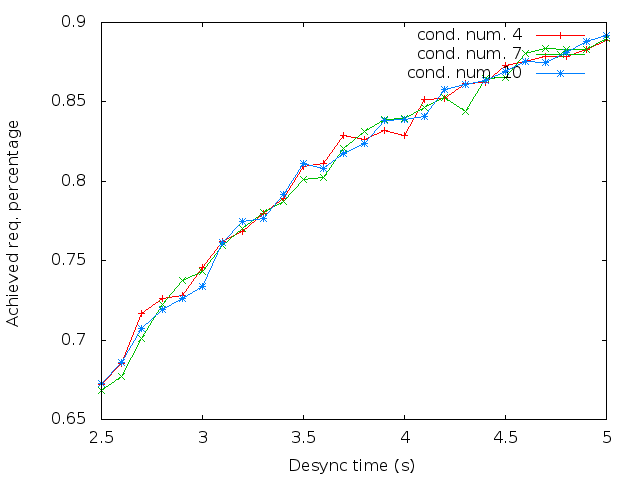
\includegraphics[width=0.4\textwidth]{hexagonsimulation/achievedlocreq4preempt1drop1speed1.png}
    \label{fig:hexagonsimulation/achievedlocreq4preempt1drop1speed1}}
    \caption{Localizzazioni riuscite}
\end{figure}

\begin{figure}[H]
    \centering
    \subfloat[Non Droponepoint]{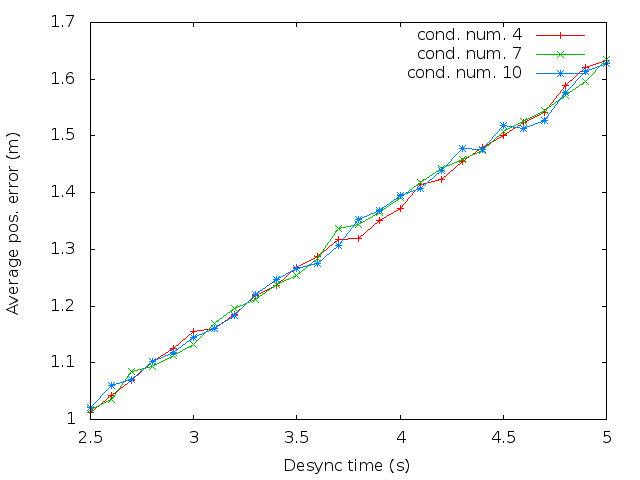
\includegraphics[width=0.4\textwidth]{hexagonsimulation/avposerrorreq3preempt1drop0speed1.png}
    \label{fig:hexagonsimulation/avposerrorreq3preempt1drop0speed1}}
    \hfill
    \subfloat[Droponepoint]{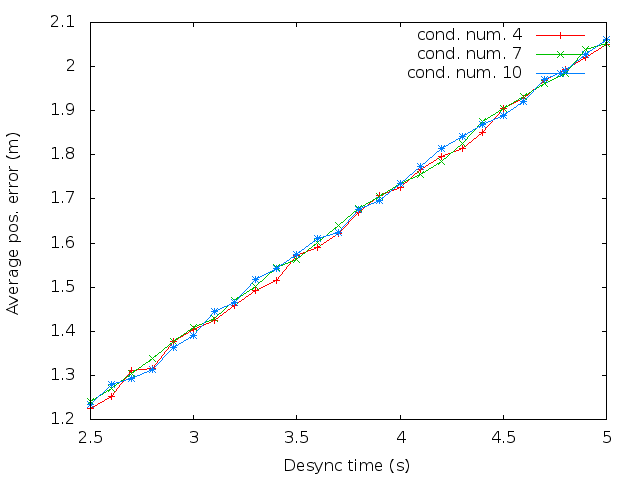
\includegraphics[width=0.4\textwidth]{hexagonsimulation/avposerrorreq4preempt1drop1speed1.png}
    \label{fig:hexagonsimulation/avposerrorreq4preempt1drop1speed1.png}}
    \caption{Errore medio}
\end{figure}

\begin{figure}[H]
    \centering
    \subfloat[Non Droponepoint]{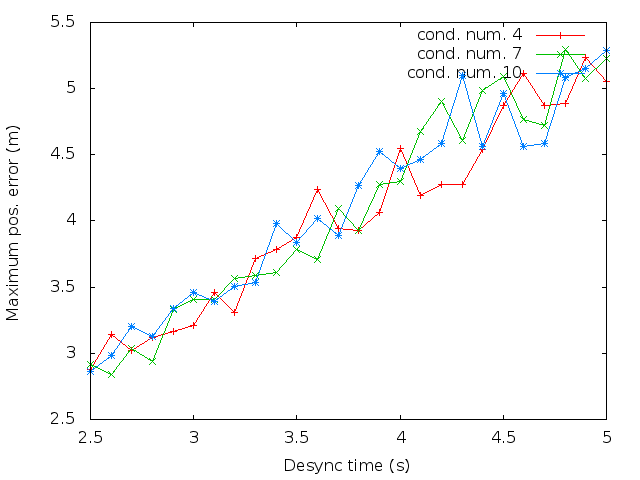
\includegraphics[width=0.4\textwidth]{hexagonsimulation/maxposerrorreq3preempt1drop0speed1.png}
    \label{fig:hexagonsimulation/maxposerrorreq3preempt1drop0speed1}}
    \hfill
    \subfloat[Droponepoint]{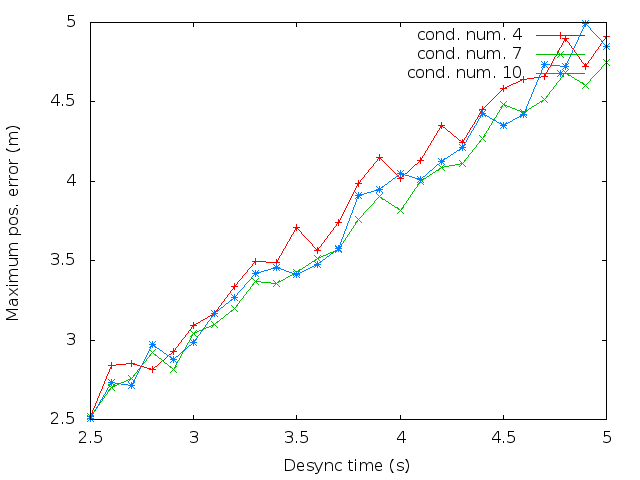
\includegraphics[width=0.4\textwidth]{hexagonsimulation/maxposerrorreq4preempt1drop1speed1.png}
    \label{fig:hexagonsimulation/maxposerrorreq4preempt1drop1speed1}}
    \caption{Errore massimo}
\end{figure}
La soglia impostata a 3 risposte fa si che la percentuale di richieste di localizzazione riuscite con questo valore sia piu' alto, almeno per quanto riguarda i grafici per numero di condizionamento 7 e 10, rispetto alla percentuale per la soglia impostata a 4 risposte (quest'ultima percentuale e', tra l'altro, incrementata dalla modalita' "droponepoint").
Nel confronto degli errori le due configurazioni mostrano profonde differenze. In primis, configurazione "preemptive"-3 risposte riesce ad ottenere un 80\% e piu' di localizzazioni riuscite con un tempo di desincronizzazione minino di 2.5 $s$, al contrario dei circa 3.5 $s$ necessari all'altra configurazione. Per questi valori, i grafici a sinistra riportano un errore medio di circa 1 $m$ (con errore massimo di poco meno di 3 $m$), mentre la modalita' "droponepoint" genera un errore medio di circa 1.5 $m$ ed errore massimo di 3.5 $m$.
Oltre ad ottenre un guadagno di precisione di circa 0.5 $m$, la configurazione mostrata nei grafici a sinistra arriva a questo risultato risparmiando all'incirca 1 $s$ nel timer di desincronizzazione dei nodi fissi (il che permette nel lungo periodo di effettuare richieste di localizzazione con piu' frequenza).
Riportiamo il confronto fra le stesse identiche configurazioni, portando la velocita' a 2 $\frac{m}{s}$.

\begin{figure}[H]
    \centering
    \subfloat[Non Droponepoint]{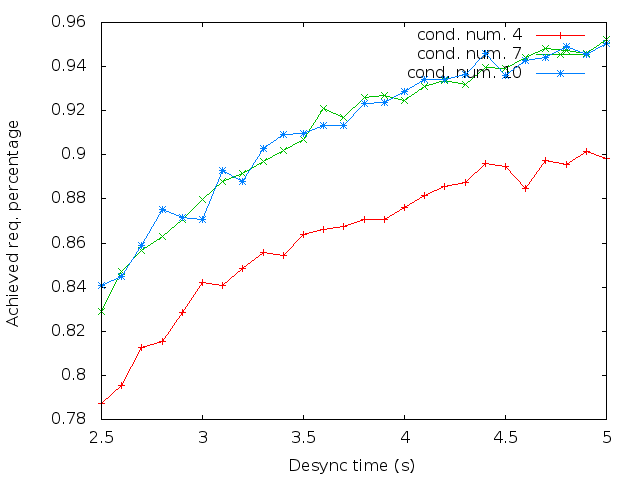
\includegraphics[width=0.4\textwidth]{hexagonsimulation/achievedlocreq3preempt1drop0speed2.png}
    \label{fig:hexagonsimulation/achievedlocreq3preempt1drop0speed2}}
    \hfill
    \subfloat[Droponepoint]{\includegraphics[width=0.4\textwidth]{hexagonsimulation/achievedlocreq4preempt1drop1speed2.png}
    \label{fig:hexagonsimulation/achievedlocreq4preempt1drop1speed2}}
    \caption{Localizzazioni riuscite}
\end{figure}

\begin{figure}[H]
    \centering
    \subfloat[Non Droponepoint]{\includegraphics[width=0.4\textwidth]{hexagonsimulation/avposerrorreq3preempt1drop0speed2.png}
    \label{fig:hexagonsimulation/avposerrorreq3preempt1drop0speed2}}
    \hfill
    \subfloat[Droponepoint]{\includegraphics[width=0.4\textwidth]{hexagonsimulation/avposerrorreq4preempt1drop1speed2.png}
    \label{fig:hexagonsimulation/avposerrorreq4preempt1drop1speed2.png}}
    \caption{Errore medio}
\end{figure}

\begin{figure}[H]
    \centering
    \subfloat[Non Droponepoint]{\includegraphics[width=0.4\textwidth]{hexagonsimulation/maxposerrorreq3preempt1drop0speed2.png}
    \label{fig:hexagonsimulation/maxposerrorreq3preempt1drop0speed2}}
    \hfill
    \subfloat[Droponepoint]{\includegraphics[width=0.4\textwidth]{hexagonsimulation/maxposerrorreq4preempt1drop1speed2.png}
    \label{fig:hexagonsimulation/maxposerrorreq4preempt1drop1speed2}}
    \caption{Errore massimo}
\end{figure}

Come si nota, modificando la velocita', non mutano le caratteristiche e le differenze fra le due configurazioni. Di nuovo, la configurazione con soglia minima di risposte impostata a 3 e modalita' "preemptive" attivata risulta vincente.

\subsection{Topologia a 8 nodi}
In ultimo, riportiamo i risultati per la topologia di rete comprendente 8 nodi fissi. 
Come per le altre topologie, presentiamo inizialmente la configurazione con AUV fermo al "centro" della costellazione dei nodi fissi. La soglia minima di risposte richiesta e' pari a 3 e ne' la modalita' "preemptive" ne' quella "droponepoint" sono attivate:
\begin{figure}[H]
    \centering
    \includegraphics[scale=0.5]{octagonsimulation/achievedlocreq3preempt0drop0speed0.png}
    \caption{Percentuale localizzazioni riuscite}
    \label{fig:octagonsimulation/achievedlocreq3preempt0drop0speed0}
\end{figure}
\begin{figure}[H]
    \centering
    \includegraphics[scale=0.5]{octagonsimulation/avposerrorreq3preempt0drop0speed0.png}
    \caption{Errore medio}
    \label{fig:octagonsimulation/avposerrorreq3preempt0drop0speed0}
\end{figure}
\begin{figure}[H]
    \centering
    \includegraphics[scale=0.5]{octagonsimulation/maxposerrorreq3preempt0drop0speed0.png}
    \caption{Errore massimo}
    \label{fig:octagonsimulation/maxposerrorreq3preempt0drop0speed0}
\end{figure}
Come gia' evidenziato per la figura ~\ref{fig:hexagonsimulation/achievedlocreq3preempt0drop0speed0}(topologia a 6 nodi), risulta accentuata la differenza fra i grafici corrispondenti a valori-soglia diversi per il numero di condizionamento. In particolare, in figura \ref{fig:octagonsimulation/achievedlocreq3preempt0drop0speed0}, notiamo una differenziazione fra i grafici ottenuti rispettivamenti con numero di condizionamento massimo pari a 7 e 10. La topologia ad 8 nodi fa si che l'angolo massimo fra 3 nodi consecutivi sia di 135 gradi (rispetto ai 120 della topologia a 6 nodi), incrementando quindi il grado di collinearita' dei nodi, e dunque il valore medio del numero di condizionamento, di un'entita' tale da far si che anche stabilendo il valore 7 come massimo per il parametro in questione alcune richieste di localizzazione non vadano a buon fine a causa del superamento di tale soglia.
Tutti e tre i grafici concludono la loro curva (valore 5 $s$ del tempo massimo di desincronizzazione) a percentuali piu' elevate rispetto alle altre due topologie (l'aggiunta di altri 2 nodi fissi fa si che sia piu' probabile ricevere le 3 risposte che mi servono per effettuare la localizzazione). In particolare, e' notevole il fatto che  con numero di condizionamento pari a 10 si superi la percentuale del 97\% di successi, sfiorando la situazione ideale del 100\% di risultati positivi.
Per quanto riguarda l'errore medio, otteniamo dei valori estremamente precisi. Di piu' , rispetto alle altre topologie si denota un andamento decrescente dell'errore medio con l'aumentare del valore del timer di desincronizzazione, imputabile all'aumento di precisione del calcolo dovuto al maggior numero di risposte ricevute (ci aspetteremmo un andamento del genere ancora piu' marcato incrementando ulteriormente il numero di nodi fissi della rete).
L'errore massimo sul posizionamento e' molto ridotto per numero di condizionamento uguale a 4 (circa 12.5 $cm$), mentre negli altri due grafici si alza a circa 40 $cm$, mostrando un lieve andamento decrementale.
Aumentanre la soglia minima di risposte richieste non comporta un miglioramento netto delle prestazioni del protocollo, mentre diminuisce ovviamente la percentuale di localizzazioni riuscite.
Passiamo ora a considerare l'AUV in movimento (dapprima 1 $\frac{m}{s}$).
Confrontiamo i risultati ottenuti con soglia minima di risposte impostata a 3, utilizzando o meno la modalita' preemptive.
\begin{figure}[H]
    \centering
    \subfloat[Non Preemptive]{\includegraphics[width=0.4\textwidth]{octagonsimulation/achievedlocreq3preempt0drop0speed1.png}
    \label{fig:octagonsimulation/achievedlocreq3preempt0drop0speed1}}
    \hfill
    \subfloat[Preemptive]{\includegraphics[width=0.4\textwidth]{octagonsimulation/achievedlocreq3preempt1drop0speed1.png}
    \label{fig:octagonsimulation/achievedlocreq3preempt1drop0speed1}}
    \caption{Localizzazioni riuscite}
\end{figure}

\begin{figure}[H]
    \centering
    \subfloat[Non Preemptive]{\includegraphics[width=0.4\textwidth]{octagonsimulation/avposerrorreq3preempt0drop0speed1.png}
    \label{fig:octagonsimulation/avposerrorreq3preempt0drop0speed1}}
    \hfill
    \subfloat[Preemptive]{\includegraphics[width=0.4\textwidth]{octagonsimulation/avposerrorreq3preempt1drop0speed1.png}
    \label{fig:octagonsimulation/avposerrorreq3preempt1drop0speed1}}
    \caption{Errore medio}
\end{figure}

\begin{figure}[H]
    \centering
    \subfloat[Non Preemptive]{\includegraphics[width=0.4\textwidth]{octagonsimulation/maxposerrorreq3preempt0drop0speed1.png}
    \label{fig:octagonsimulation/maxposerrorreq3preempt0drop0speed1}}
    \hfill
    \subfloat[Preemptive]{\includegraphics[width=0.4\textwidth]{octagonsimulation/maxposerrorreq3preempt1drop0speed1.png}
    \label{fig:octagonsimulation/maxposerrorreq3preempt1drop0speed1}}
    \caption{Errore massimo}
\end{figure}
Vediamo come fra la modalita' preemptive e quella normale vi sia una netta differenza per quanto riguarda il numero di localizzazioni andate a buon fine per quanto riguarda le simulazioni effettuate con soglia del numero di condizionamento pari a 4. La modalita' preemptive causa la drastica diminuzione delle localizzazioni riuscite (e' piu' probabile che le 3 risposte ricevute dall'AUV siano da nodi vicini tra loro e quindi abbastanza allineati), mentre la modalita' di funzionamento normale presenta dei valori simili alla configurazione con AUV fermo (\ref{fig:octagonsimulation/achievedlocreq3preempt0drop0speed0}).
In entrambe le configurazioni, nei grafici per i valori soglia del numero di condizionamento 7 o 10 le richieste di posizionamento riuscite partono da un valore superiore all'85\% , con tempo di desincronizzazione dei nodi fissi pari a 2.5 $s$.
Per questi valori, la modalita' preemptive genera un errore medio di circa 1 $m$ ed un errore massimo di 3.5 $m$. La modalita' di funzionamento normale invece effettua il calcolo delle coordinate dell'AUV con un errore medio di piu' di 2 $m$ ed un errore massimo di piu' di 4 $m$.
All'aumentare del tempo di desincronizzazione, il comportamento delle due modalita' differisce ulteriormente. L'errore medio della modalita' preemptive aumenta ma non in maniera decisiva, toccando il valore di quasi 1.5 $m$ per timer di desincronizzazione pari a 5 $s$, mentre l'errore medio nella modalita' normale sale a circa 3.5 $m$. Per la modalita' preemptive questo e' giustificato dal fatto che, pur aumentando il valore del timer, non appena il veicolo riceve 3 risposte effettua il calcolo della propria posizione. Essendoci 8 nodi fissi da cui poter ricevere risposta, cio' non avviene molto tempo dopo l'avvio del timer. Al contrario, nella modalita' normale l'aumento del tempo massimo di desincronizzazione causa l'effettiva dilatazione del tempo che intercorre tra l'arrivo delle risposte e l'avvio del calcolo delle coordinate (aumentando notevolmente l'errore del calcolo).
Riportiamo ora la configurazione in cui il nodo si muove sempre a velocita' di 1 $\frac{m}{s}$ , la soglia minima di risposte e' impostata a 4 nodi e sono attivate sia la modalita' "preemptive" che quella "droponepoint". 
\begin{figure}[H]
    \centering
    \includegraphics[scale=0.5]{octagonsimulation/achievedlocreq4preempt1drop1speed1.png}
    \caption{Percentuale localizzazioni riuscite}
    \label{fig:octagonsimulation/achievedlocreq4preempt1drop1speed1}
\end{figure}
\begin{figure}[H]
    \centering
    \includegraphics[scale=0.5]{octagonsimulation/avposerrorreq4preempt1drop1speed1.png}
    \caption{Errore medio}
    \label{fig:octagonsimulation/avposerrorreq4preempt1drop1speed1}
\end{figure}
\begin{figure}[H]
    \centering
    \includegraphics[scale=0.5]{octagonsimulation/maxposerrorreq4preempt1drop1speed1.png}
    \caption{Errore massimo}
    \label{fig:octagonsimulation/avposerrorreq4preempt1drop1speed1}
\end{figure}
Come evidente dai grafici, non c'e' molta differenza con la configurazione al minimo di 3 risposte precedentemente esposta.
In ultimo, confrontiamo i risultati ottenuti con velocita' dell'AUV  di 2 $\frac{m}{s}$. Utilizziamo di base la modalita' "preemptive". Compariamo i risultati avendo in un caso la soglia minima di risposte a 3, mentre nell'altro impostata a 4 con la modalita' "droponepoint" attivata.
\begin{figure}[H]
    \centering
    \subfloat[3 risposte]{\includegraphics[width=0.4\textwidth]{octagonsimulation/achievedlocreq3preempt1drop0speed2.png}
    \label{fig:octagonsimulation/achievedlocreq3preempt1drop0speed2}}
    \hfill
    \subfloat[4 risposte]{\includegraphics[width=0.4\textwidth]{octagonsimulation/achievedlocreq4preempt1drop1speed2.png}
    \label{fig:octagonsimulation/achievedlocreq4preempt1drop1speed2}}
    \caption{Localizzazioni riuscite}
\end{figure}

\begin{figure}[H]
    \centering
    \subfloat[3 risposte]{\includegraphics[width=0.4\textwidth]{octagonsimulation/avposerrorreq3preempt1drop0speed2.png}
    \label{fig:octagonsimulation/avposerrorreq3preempt1drop0speed2}}
    \hfill
    \subfloat[4 risposte]{\includegraphics[width=0.4\textwidth]{octagonsimulation/avposerrorreq4preempt1drop1speed2.png}
    \label{fig:octagonsimulation/avposerrorreq4preempt1drop1speed2}}
    \caption{Errore medio}
\end{figure}

\begin{figure}[H]
    \centering
    \subfloat[3 risposte]{\includegraphics[width=0.4\textwidth]{octagonsimulation/maxposerrorreq3preempt1drop0speed2.png}
    \label{fig:octagonsimulation/maxposerrorreq3preempt1drop0speed2}}
    \hfill
    \subfloat[4 risposte]{\includegraphics[width=0.4\textwidth]{octagonsimulation/maxposerrorreq4preempt1drop1speed2.png}
    \label{fig:octagonsimulation/maxposerrorreq4preempt1drop1speed2}}
    \caption{Errore massimo}
\end{figure}
I risultati ottenuti sono molto simili a quelli per la topologia a 6 nodi (\ref{fig:hexagonsimulation/achievedlocreq3preempt1drop0speed2}, \ref{fig:hexagonsimulation/avposerrorreq3preempt1drop0speed2}, \ref{fig:hexagonsimulation/maxposerrorreq3preempt1drop0speed2}).


\section{Conclusioni}
Per quanto riguarda la configurazione economicamente piu' facilmente approntabile (quella con 4 nodi fissi), abbiamo ottenuto dei risultati abbastanza incoraggianti. Con l'AUV fermo, la precisione garantita di circa 10 $cm$ rende il protocollo  affidabile per un utilizzo concreto, considerando che nelle prove sul campo l'errore ottenuto sara' sicuramente piu' alto ma non troppo distante da questo valore notevolmente contenuto.
Risulta essere non ottimale, invece, la percentuale di localizzazioni andate a buon fine (nelle simulazioni non si e' riuscito a superare il  70\%). Considerando, invece, l'AUV in movimento, possiamo ritenere una percentuale di posizionamenti riusciti al 80\% un ottimo risultato e, per questo valore, otteniamo un errore medio di 1.7 $m$ ed uno massimo di circa 4 $m$. Se pensiamo alla missione simulata dal veicolo, ovvero il "monitoraggio" di un area quadrata di circa 200 $m$ di lato, l'accuratezza della posizione calcolata e' abbastanza accetabile. In situazioni del genere e' anche possibile, oltre a correggere il posizionamento grazie all'introduzione di tecniche di dead reckoning, fare in modo di fermare il veicolo, con una certa cadenza, e calcolarne le coordinate da fermo in maniera precisa, per poi riprendere lo svolgimento della missione.
\newline
Ovviamente, incrementando nodi fissi si ottengono risultati piu' precisi, ma per la velocita' di 1 $\frac{m}{s}$ il miglioramento rispetto alla topologia a 4 nodi non e' forse tale da giustificare il deployment di un maggion numero di nodi.
Ad esempio, con 8 nodi potremmo ottenere la precisione di circa 1 $m$ con il 90\% di localizzazioni riuscite, ovvero miglioreremmo la precisione rispetto alla configurazione con la meta' dei nodi di solamente 70 $cm$ (la percentuale di successo del 10\%) raddoppiando il costo del network necessario.
Diverso e' il discorso se la missione di un veicolo mobile richiede che esso si sposti a velocita' piu' elevate. I risultati ottenuti simulando il movimento dell'AUV a 2 $\frac{m}{s}$ mostrano notevoli differenze rispetto al numero di nodi fissi impiegati nella rete.
Con la topologia a 4 nodi, il risultato migliore che otteniamo e' un errore medio sulla posizione di 2.8 $m$ (errore massimo di 8 $m$), con percentuale di localizzazione riuscite dell'80\% e valore del timer di desincronizzazione pari a 4.5 $s$.
Aggiungendo due nodi alla topologia, l'errore medio scende a 1.65 $m$ e quello massimo a 5.5 $m$. Inoltre, la percentuale di localizzazioni andate a buon fine sale oltre l'80\% (circa l'83\%), con un tempo di desincronizzazione dei nodi fissi pari a 2.5 $s$, due secondi in meno rispetto alla topologia a 4 nodi. Cio' rappresenta un enorme guadagno in termini di accuratezza e precisione, oltre al vantaggio dovuto al minor tempo necessario alla localizzazione dell'AUV.
Utilizzando la topologia ad 8 nodi si ottengono risultati simili all'utilizzo di 6 nodi, se non che' per gli stessi valori degli errori e del timer di desincronizzazione si ottiene una percentuale di posizionamenti riusciti pari a circa il 90\%.










\backmatter

\clearpage
%% ----------------------------------------------------------------
\label{Bibliography}
\lhead{\emph{Bibliografia}}  % Change the left side page header to "Bibliography"
\nocite{*}
\printbibliography
% bibliography
%\cleardoublepage
%\phantomsection
%\bibliographystyle{sapthesis} % BibTeX style
%\bibliography{bibliography} % BibTeX database without .bib extension

\end{document}
